\subsection{李群的定义}

设 \(G\) 为一个集合。如果 \(G\) 上的群结构与解析 K-流形结构满足以下条件，则称二者相容：

(GL) 映射 \((g, h) \mapsto gh^{-1}\) 从 \(\mathbf{G} \times \mathbf{G}\) 到 \(\mathbf{G}\) 是解析的。

定义 1. K 上的李群是一个带有群结构和解析 K-流形结构的集合 G，并且这两个结构相容。

在 \(\mathbf{R}\) 上的李群称为实李群（相应地，在 \(\mathbf{C},\mathbf{Q}_p\) 上的称为复李群，在 \(p\) -进情形下称为相应的 p-进李群）。

设 \(\mathbf{G}\) 为带有解析流形结构的群。对于 \(g, h, g_0, h_0\)，它们属于 \(\mathbf{G}\)，

\[
g h ^ {- 1} = (g _ {0} h _ {0} ^ {- 1}) h _ {0} ((g _ {0} ^ {- 1} g) (h _ {0} ^ {- 1} h) ^ {- 1}) h _ {0} ^ {- 1}.\tag{1}
\]

由此可知，当且仅当以下三个条件成立时，G 是李群：

\((\mathbf{GL}_1)\) 对所有 \(g_0 \in \mathbf{G}\)，映射 \(g \mapsto g_0 g\) 从 \(\mathbf{G}\) 到 \(\mathbf{G}\) 是解析的；

\((\mathrm{GL}_2)\) 对所有 \(g_0 \in \mathbf{G}\)，映射 \(g \mapsto g_0gg_0^{-1}\) 从 \(\mathbf{G}\) 到 \(\mathbf{G}\) 在 \(e\) 的某个开邻域内是解析的；

\((\mathrm{GL}_3)\) 映射 \((g,h)\mapsto gh^{-1}\) 从 \(\mathbf{G}\times \mathbf{G}\) 到 \(\mathbf{G}\) 在 \((e,e)\) 的某个开邻域内是解析的。

设 G 为李群。对于所有 \(g \in G\)，\(\gamma(g)\) 和 \(\delta(g)\) 都是 G 的底层流形的自同构。因此该流形是纯的（Differentiable and Analytic Manifolds, R, 5.1.7）。特别地，对于所有 \(g \in G\)，G 在 g 处的维数等于 dim G（回忆 dim G 是一个 \(\geqslant 0\) 的整数或 \(+\infty\)）。

由于解析映射是连续的，李群是一个拓扑群，其底层拓扑是流形结构所给出的拓扑。设 G 为一个集合。如果 G 上的拓扑群结构与解析 K-流形结构相容，则称它们相容，并且 G 上的拓扑是流形结构的底层拓扑。

引理 1. 设 G 为李群，U 为 e 的开邻域，E 为完备赋范空间，且 \(\phi: \mathrm{U} \to \mathrm{E}\) 是流形 G 的一个图。则存在包含于 U 中的 e 的某个邻域 W，使得 \(\phi \mid W\) 是 W（带右一致结构）到 \(\phi(W)\)（带由 E 上的一致结构诱导的一致结构）的同构。

可假定 \(\phi(e) = 0\)。令 \(U' = \dot{\phi}(U)\)。令 \(\dot{\psi}: U' \to U\) 为 \(\dot{\phi}\) 的逆映射。取 \(V\) 为 \(e\) 的一个对称开邻域，使 \(V^2 \subset U\)，并令 \(V' = \dot{\phi}(V)\)。定义映射 \(\theta_1, \theta_2\)，它们从 \(V' \times V'\) 到 \(V' \times U'\)，如下：

\[
\begin{array}{l} \theta_ {1} (x, y) = (x, \phi (\psi (x) \psi (y) ^ {- 1})) \\ \theta_ {2} (x, y) = (x, \phi (\psi (y) ^ {- 1} \psi (x))). \end{array}
\]

直接验证可得，当 \(\theta_{2}(\theta_{1}(x,y)) = \theta_{1}(\theta_{2}(x,y)) = (x,y)\) 且 \(x\)、\(y\) 充分接近 0 时成立。另一方面，\(\theta_{1}\) 和 \(\theta_{2}\) 是解析的，因而在 \((0,0)\) 处严格可微。因此（Differentiable and Analytic Manifolds, R, 1.2.2），存在 0 的一个邻域 \(W'\)（在 \(V'\) 中）以及常数 \(a > 0\)、\(b > 0\)，使得

\[
\begin{array}{r l} a (\| x _ {1} - x _ {2} \| + \| \phi (\psi (x _ {1}) \psi (y _ {1}) ^ {- 1}) - \phi (\psi (x _ {2}) \psi (y _ {2}) ^ {- 1}) \|) \\ & \leqslant \| x _ {1} - x _ {2} \| + \| y _ {1} - y _ {2} \| \\ & \leqslant b (\| x _ {1} - x _ {2} \| + \| \phi (\psi (x _ {1}) \psi (y _ {1}) ^ {- 1}) - \phi (\psi (x _ {2}) \psi (y _ {2}) ^ {- 1}) \|) \end{array}
\]

对 \(x_1, x_2, y_1, y_2\) 在 \(W'\) 中均成立。令 \(x_1 = x_2 = y_2\)，得到

\[
a \| \phi (\psi (x _ {1}) \psi (y _ {1}) ^ {- 1}) \| \leqslant \| x _ {1} - y _ {1} \| \leqslant b \| \phi (\psi (x _ {1}) \psi (y _ {1}) ^ {- 1}) \|.\tag{2}
\]

对于 \(\delta > 0\)，令 \(\mathrm{N}_{\delta}\) 为 \((x,y)\in W'\times W'\) 中满足 \(\| x - y\| \leqslant \delta\) 的有序对。各 \(\mathrm{N}_{\delta}\) 构成 \(W'\) 中围的基本系。记 \(W = \psi(W')\)。令 \(\mathrm{M}_{\delta}\) 为 \((u,v)\in W\times W\) 中满足 \(\| \phi (u v^{-1})\| \leqslant \delta\) 的有序对。各 \(\mathrm{M}_{\delta}\) 构成带右一致结构的 \(W\) 中围的基本系。但关系 (2) 表明

\[
\mathrm{N} _ {\delta} \subset (\phi \times \phi) (\mathrm{M} _ {a ^ {- 1} \delta}), \quad (\phi \times \phi) (\mathrm{M} _ {\delta}) \subset \mathrm{N} _ {b \delta}
\]

因此 W 具有引理所述的性质。

命题 1. 李群是完备可度量拓扑群。

由于 \(e\) 有一个同胚于赋范空间开球的开邻域，\(e\) 有一个交为 \(\{e\}\) 的可数基本邻域系。因此 G 是可度量的（General Topology, Chapter III, § 1, Corollary to Proposition 2 and Chapter IX, § 3, Proposition 1）。由引理 1，存在 \(e\) 的一个邻域，它在右一致结构下是完备的，从而 G 是完备的（General Topology, Chapter III, § 3, Proposition 4。

命题 2. 设 G 为李群。

\begin{enumerate}
\def\labelenumi{(\roman{enumi})}
\item
  如果 \(\mathbf{K} = \mathbf{R}\) 或 \(\mathbf{C}\)，则 \(\mathbf{G}\) 局部连通。
\item
  如果 \(\mathbf{K}\) 不同于 \(\mathbf{R}\) 和 \(\mathbf{C}\)，则 \(\mathbf{G}\) 是零维的（General Topology, Chapter IX, § 6, Definition 5）。
\item
  设 K 局部紧。G 局部紧的充要条件是 G 是有限维的。
\item
  如果 \(\mathbf{G}\) 由一个拓扑具有可数基的子空间生成，则 \(\mathbf{G}\) 的拓扑具有可数基。
\end{enumerate}

令 U 为 \(e\) 的一个邻域。存在 \(\mathbf{U}_1\)，它是 \(e\) 的一个开邻域，包含于 U 中，且同胚于 K 上某个赋范空间 E 的开球。如果 \(\mathbf{K} = \mathbf{R}\) 或 \(\mathbf{C}\)，则 \(\mathbf{U}_1\) 是连通的，这证明了 (i)。设 K 是超度量的。存在 \(\mathbf{U}_2\)，它是 \(e\) 的一个邻域，在 G 中是闭的且满足 \(\mathbf{U}_2 \subset \mathbf{U}_1\)。于是存在 \(\mathbf{U}_3\)，它是 \(e\) 的一个邻域，满足 \(\mathbf{U}_3 \subset \mathbf{U}_2\)，且 \(\mathbf{U}_3\) 对 \(\mathbf{U}_1\) 是开且闭的。于是 \(\mathbf{U}_3\) 对 \(\mathbf{U}_2\) 是闭的，因而对 G 也是闭的；并且对 \(\mathbf{U}_1\) 是开的，因而对 G 也是开的。这证明了 (ii)。G 局部紧的充要条件是 E 局部紧；若 K 局部紧，这等价于 E 是有限维的（Topological Vector Spaces, Chapter I, § 2, Theorem 3），从而得到 (iii)。设 G 由子集 V 生成，并令 \(W = V \cup V^{-1}\)；于是

\[
G = W \cup W ^ {2} \cup W ^ {3} \cup \dots ;
\]

如果 V 中存在一个稠密序列，则可见 G 中存在一个稠密序列，而由于 G 是可度量的（命题 1），G 的拓扑具有可数基。

推论。如果 K = R 或 C，且 G 连通并且有限维，则 G 局部连通且局部紧，并且其拓扑具有可数基。

引理 2. 设 X 是 \(\mathbf{C}^r\) 类流形，\(e\) 是 X 中的一点，U、V 是 \(e\) 的开邻域，且 \(m\) 是一个 \(\mathbf{C}^r\) 类映射，从 \(\mathrm{U} \times \mathrm{U}\) 到 X，满足以下条件：

\begin{enumerate}
\def\labelenumi{(\alph{enumi})}
\item
  \(m(e,x) = m(x,e) = x\) 对所有 \(x\in \mathbf{U}\) 成立；
\item
  \(\mathrm{V} \subset \mathrm{U}\)，\(m(\mathrm{V} \times \mathrm{V}) \subset \mathrm{U}\)，并且 \(m(m(x, y), z) = m(x, m(y, z))\) 对 \(x, y, z\) 属于 \(\mathrm{V}\) 时成立。
\end{enumerate}

则存在 \(e\) 的一个开邻域 W（在 V 中）以及 W 的一个流形自同构 \(\theta\)，使得 \(\theta(e) = e\)、\(\theta(\theta(x)) = x\)，并且 \(m(x, \theta(x)) = m(\theta(x), x) = e\) 对所有 \(x \in W\) 成立。

\(m(e,y) = y\) 对所有 \(y \in \mathrm{U}\) 成立，因此由隐函数定理，存在一个开邻域 \(\mathrm{W}_1\)，它是 \(e\) 在 \(\mathrm{V}\) 中的邻域，并存在一个映射 \(\theta_1\)，它是一个 \(C^r\) 类映射，从 \(\mathrm{W}_1\) 到 \(\mathrm{V}\)，使得 \(\theta_1(e) = e\)，且 \(m(x,\theta_1(x)) = e\) 对所有 \(x \in \mathrm{W}_1\) 成立。类似地，存在一个开邻域 \(\mathrm{W}_2\)，它是 \(e\) 在 \(\mathrm{V}\) 中的邻域，并存在一个映射 \(\theta_2\)，它是一个 \(C^r\) 类映射，从 \(\mathrm{W}_2\) 到 \(\mathrm{V}\)，使得 \(\theta_2(e) = e\)，且 \(m(\theta_2(x),x) = e\) 对所有 \(x \in \mathrm{W}_2\) 成立。对于 \(x \in \mathrm{W}_1 \cap \mathrm{W}_2\)。

\[
\begin{array}{r l} \theta_ {2} (x) & = m (\theta_ {2} (x), e) = m (\theta_ {2} (x), m (x, \theta_ {1} (x))) \\ & = m (m (\theta_ {2} (x), x), \theta_ {1} (x)) = m (e, \theta_ {1} (x)) = \theta_ {1} (x). \end{array}
\]

令 \(\theta(x)\) 为 \(\theta_1(x)\) 与 \(\theta_2(x)\) 对于 \(x \in W_1 \cap W_2\) 的公共值。令 \(W\) 为 \(x \in W_1 \cap W_2\) 中满足 \(\theta(x) \in W_1 \cap W_2\) 的点的集合。集合 \(W\) 是开集。对于 \(x \in W\)，

\[
\theta (\theta (x)) = m (m (x, \theta (x)), \theta (\theta (x))) = m (x, m (\theta (x), \theta (\theta (x)))) = m (x, e) = x
\]

从而 \(\theta(x) \in W\)。可见 \(\theta \mid W\) 定义了流形 \(W\) 的一个自同构。

命题 3. 设 \(\mathbf{X}\) 为解析流形，\(m\) 为 \(\mathbf{X}\) 上具有单位元的解析结合复合律。可逆元集合 \(\mathbf{G}\) 属于 \(\mathbf{X}\) 且在 \(\mathbf{X}\) 中是开集，并且 \(\mathbf{G}\) 配以 \(m \mid (\mathbf{G} \times \mathbf{G})\) 和由 \(\mathbf{X}\) 诱导的流形结构后是李群。

由引理 2，G 是单位元的一个邻域。对于所有 \(g \in \mathbb{G}\)，映射 \(x \mapsto m(g, x)\) 是流形 X 的自同构。因此 G 在此映射下的像是 \(g\) 的一个邻域，显然包含于 G 中。所以 G 在 X 中是开集。显然条件 \((\mathrm{GL}_1)\) 和 \((\mathrm{GL}_2)\) 成立。条件 \((\mathrm{GL}_3)\) 由引理 2 得出。

\subsection*{李群的例子}

\begin{enumerate}
\def\labelenumi{(\arabic{enumi})}
\tightlist
\item
  令 \(\mathbf{E}\) 为 \(\mathbf{K}\) 上的完备可赋范空间。映射 \((x, y) \mapsto x - y\) 从 \(\mathbf{E} \times \mathbf{E}\) 到 \(\mathbf{E}\)，是连续线性的，因而是解析的。
\end{enumerate}

因此，E 配以其加法群结构和解析流形结构后是李群。

特别地，K 是李群。

\begin{enumerate}
\def\labelenumi{(\arabic{enumi})}
\setcounter{enumi}{1}
\tightlist
\item
  令 A 为 K 上的完备可赋范含单位结合代数。从 A × A 到 A 的乘法 \((x,y)\mapsto xy\) 是双线性且连续的，因而是解析的。命题 3 表明，A 的可逆元群 A* 在 A 中是开集（这也可由 General Topology, Chapter IX, §3, Proposition 13 得到），并且 A* 是李群。
\end{enumerate}

例如，设 E 为 K 上的完备可赋范空间，并令 A = \(\mathcal{L}(\mathrm{E})\)（General Topology, Chapter IX, § 3, Proposition 5）。于是 A* 是 E 的自同构群 GL(E)。因此，这个群自然地带有 K 上的李群结构。更具体地说，GL(n, K) 配以由 \(\mathbf{M}_{n}(\mathbf{K})\) 诱导的流形结构后是李群。对于 \(n = 1\)，可见乘法群 K* 配以由 K 诱导的流形结构后是李群。

\begin{enumerate}
\def\labelenumi{(\arabic{enumi})}
\setcounter{enumi}{2}
\tightlist
\item
  令 G 为 K 上的李群。令 \(K' = R\) 或 C 或一个非离散完备超度量域，并令 \(\sigma\) 为赋值域 \(K'\) 到 K 的一个赋值子域上的同构。于是 G 配以通过限制标量得到的 K'-流形结构后，是 \(K'\) 上的李群；称其为由李群 G 通过限制标量导出的李群（从 K 到 \(K'\) 通过 \(\sigma\)）。例如，每个复李群都自然地带有实李群结构。此外，每个复李群 G 都关联着一个称为 G 的共轭的复李群，它由 C 的自同构 \(z \mapsto \bar{z}\) 从 G 导出。
\end{enumerate}

\subsection{李群的态射}

定义 2. 设 G 和 H 为李群。G 到 H 的李群态射（若无混淆也简称 G 到 H 的态射）是一个从 G 到 H 的映射，它是群同态且解析。G 的自同构群记为 Aut(G)。

G 的恒等映射是态射。两个态射的复合是态射。如果 \(f: G \to H\) 和 \(f': H \to G\) 是互逆的两个态射，则 f 和 \(f'\) 是李群同构。

例。（1）设 \(G\) 为李群。对于所有 \(x \in G\)，\(\operatorname{Int}(x)\) 都是李群 \(G\) 的自同构。

\begin{enumerate}
\def\labelenumi{(\arabic{enumi})}
\setcounter{enumi}{1}
\item
  设 G 为李群。令 \(G^{\nu}\) 表示 G 的对立群，并赋予与 G 相同的流形结构。显然 \(G^{\nu}\) 是李群（称为 G 的对立李群），且映射 \(g \mapsto g^{-1}\) 是从李群 G 到李群 \(G^{\nu}\) 的同构。
\item
  设 G 为李群，E 为完备可赋范空间。G 在 E 上的解析线性表示（若无混淆也简称 G 在 E 上的线性表示）是从李群 G 到李群 \(\mathbf{GL}(\mathrm{E})\) 的态射，换言之，是一个解析映射 \(\pi\)，从 \(\mathbf{G}\) 到 \(\mathbf{GL}(\mathrm{E})\)，满足 \(\pi (gg^{\prime}) = \pi (g)\pi (g^{\prime})\) 对 \(g\)、\(g^{\prime}\) 属于 \(\mathbf{G}\) 成立。设 E 在 K 上有有限基 \((e_1,e_2,\ldots ,e_n)\)；令 \((e_1^*,e_2^*,\dots ,e_n^*)\) 为对偶基；令 \(\rho\) 为从群 G 到群 \(\mathbf{GL}(\mathrm{E})\) 的同态；则以下条件等价：
\end{enumerate}

\begin{enumerate}
\def\labelenumi{(\roman{enumi})}
\item
  \(\rho\) 是解析线性表示；
\item
  对所有 \(x \in \mathbf{E}\) 和 \(x' \in \mathbf{E}'\)，函数 \(g \mapsto \langle \rho(g)x, x' \rangle\) 在 \(\mathbf{G}\) 上是解析的；
\item
  对所有 \(i\) 和 \(j\)，函数 \(g \mapsto \langle \rho(g)e_i, e_j^*\rangle\) 在 G 上是解析的。蕴含关系 (i) \(\Rightarrow\) (ii) \(\Rightarrow\) (iii) 显然。另一方面，函数 \(u \mapsto \langle ue_i, e_j^*\rangle\) 在 \(\mathcal{L}(\mathrm{E})\) 上构成坐标系；因此它们限制到 \(\mathbf{GL}(\mathrm{E})\) 后在 \(\mathbf{GL}(E)\) 上构成坐标系，从而得到蕴含关系 (iii) \(\Rightarrow\) (i)。
\end{enumerate}

设 G 为实李群，E 为实完备可赋范空间，且 \(\rho\) 是从群 G 到群 \(\mathbf{GL}(\mathbf{E})\) 的同态。我们将在§8、定理 1 中看到，如果 \(\rho\) 连续（当 \(\mathbf{GL}(\mathbf{E})\) 带有由 \(\mathrm{L}(\mathbf{E})\) 上的范数导出的拓扑时），那么 \(\rho\) 是解析的。但请注意，这里的连续性概念不同于 Integration, 第 VIII 章，第 2 节，定义 1 (ii)（练习 1）中所考虑的概念。

\begin{enumerate}
\def\labelenumi{(\arabic{enumi})}
\setcounter{enumi}{3}
\tightlist
\item
  设 G 为实李群，E 为复完备可赋范空间。G 在 E 上的解析线性表示是 G 到 \(\mathbf{GL}(\mathrm{E})\) 的底层实李群的态射。
\end{enumerate}

命题 4. 设 G 和 H 为李群，f 为从群 G 到群 H 的同态。f 解析的充要条件是存在 G 的一个非空开子集 U，使得 \(f \mid U\) 是解析的。

该条件显然是必要的。设它成立。对于所有 \(x_0 \in G\)，\(f(x_0x) = f(x_0)f(x)\) 对所有 \(x \in U\) 成立，因此 \(f|_{x_0U}\) 是解析的。但各集合 \(x_0U\)（其中 \(x_0 \in G\)）构成 \(G\) 的一个开覆盖。

备注。若 \(f\) 在 \(e\) 处是浸入（相应地，在 \(e\) 处是浸没），显然 \(f\) 是浸入（相应地是浸没）。

\subsection{李子群}

设 G 为李群，H 为 G 的子群，同时也是 G 的子流形。则映射 \((x,y)\mapsto xy^{-1}\) 从 \(H\times H\) 到 G 是解析的，因此映射 \((x,y)\mapsto xy^{-1}\) 从 \(H\times H\) 到 H 也是解析的。（Differentiable and Analytic Manifolds, R, 5.8.5）。因此 H 配以由 G 的群结构和流形结构诱导的结构后是李群。

定义 3. 设 G 为李群。如果 G 的子集 H 是 G 的子群和子流形，则称 H 为李子群。

G 的开子群是 G 的李子群。特别地，如果 G 是实或复李群，则其单位元连通分支是 G 的李子群。

命题 5. 设 G 为李群，H 为 G 的李子群。

\begin{enumerate}
\def\labelenumi{(\roman{enumi})}
\item
  H 在 G 中是闭的。
\item
  H 到 G 的典范嵌入是李群态射。
\item
  设 \(\mathbf{L}\) 为李群，\(f\) 为从 \(\mathbf{L}\) 到 \(\mathbf{G}\) 的映射，满足 \(f(\mathbf{L}) \subset \mathbf{H}\)。要使 \(f\) 成为从 \(\mathbf{L}\) 到 \(\mathbf{H}\) 的态射，充要条件是 \(f\) 是从 \(\mathbf{L}\) 到 \(\mathbf{G}\) 的态射。
\end{enumerate}

由 Differentiable and Analytic Manifolds, R, 5.8.3，H 是局部闭的。因此 H 是闭的（General Topology, Chapter III, § 2, Proposition 4）。断言 (ii) 显然。断言 (iii) 由 Differentiable and Analytic Manifolds, R, 5.8.5 得出。

命题 6. 设 G 为李群，H 为 G 的子群。H 是 G 的李子群的充要条件是：存在一点 \(h \in H\) 以及 G 中 h 的一个开邻域 U，使 \(H \cap U\) 是 G 的子流形。

该条件显然是必要的。设它成立。对于所有 \(h' \in \mathbf{H}\)，平移 \(\gamma (h'h^{-1})\) 是流形 \(G\) 的自同构，并将子流形 \(H \cap U\)（在 \(U\) 中）映入子流形 \((h'h^{-1}H) \cap (h'h^{-1}U)\)（在 \(h'h^{-1}U\) 中）。由于 \(h'h^{-1}H = H\)，且 \(h'h^{-1}U\) 是 \(h'\) 在 \(G\) 中的开邻域，可见 \(H\) 的每一点都有一个开邻域 \(V\)，使 \(V \cap H\) 是 \(G\) 的子流形。因此 \(H\) 是 \(G\) 的子流形。

设 \(G\) 为李群，\(H\) 为 \(G\) 的李子群。若 \(L\) 是 \(H\) 的李子群，则 \(L\) 是 \(G\) 的李子群（由 Differentiable and Analytic Manifolds, \(R\)，5.8.6）。设 \(M\) 是 \(G\) 的李子群且 \(M \subset H\)。则 \(M\) 是 \(H\) 的李子群，因为 \(M\) 到 \(H\) 的典范嵌入显然是浸入。

令 k 为 K 的一个非离散闭子域。G 的李 k-子群是 G 的底层李 k-群的李子群。

备注。若在定义 3 中以 ``子流形'' 替换 ``拟子流形''，便得到 G 的李拟子群的定义。（对于有限维 G，李拟子群恰好就是李子群。）设 K 的特征为 0。对李拟子群，命题 5 以同样的证明仍然成立。命题 6 也以同样的证明成立，只需将 ``李子群'' 替换为 ``李拟子群''，并将 ``子流形'' 替换为 ``拟子流形''。

\subsection{李群的半直积}

设 I 为有限集，\((\mathbf{L}_{i})_{i\in I}\) 为一族李群。\(L=\prod_{i\in I}L_{i}\) 上的群结构和流形结构相容，因而 L 带有李群结构。L 称为这族李群 \((\mathbf{L}_{i})_{i\in I}\) 的积李群。

设 L、M 为李群，\(\sigma\) 为从 L 到群 M 的自同构群的同态。设 S 为关于 \(\sigma\) 的 L 与 M 的外半直积（Algebra, Chapter I, §6, no. 1, Definition 2）。

命题 7. 如果映射 \((m, l) \mapsto \sigma(l)m\) 从 \(\mathbf{M} \times \mathbf{L}\) 到 \(\mathbf{M}\) 是解析的，则群 \(\mathbf{S}\) 配以 \(\mathbf{M}\) 和 \(\mathbf{L}\) 的积流形结构后是李群。

对于 L 中的 \(l, l'\) 以及 M 中的 \(m, m'\)，

\[
\begin{array}{r l} (m, l) (m ^ {\prime}, l ^ {\prime}) ^ {- 1} & = m l l ^ {- 1} m ^ {\prime - 1} = m (\sigma (l l ^ {\prime - 1}) m ^ {\prime - 1}) l l ^ {\prime - 1} \\ & = (m (\sigma (l l ^ {\prime - 1}) m ^ {\prime - 1}), l l ^ {\prime - 1}) \end{array}
\]

从而得到命题。

如果命题 7 的条件成立，则称李群 S 为关于 \(\sigma\) 的 L 与 M 的（外）半直积李群。

显然，L（相应地，M）到 S 的典范嵌入是从 L（相应地，M）到 S 的一个李子群的同构，并将该李子群与 L（相应地，M）认同。S 到 L 的典范映射是李群态射。

反之，设 G 为李群，L、M 为两个李子群，并且群 G（代数上）是 L 与 M 的半直积（Algebra, Chapter I, § 6, no. 1）。记 \(\sigma(l)m = lml^{-1}\)，其中 \(l \in L\) 且 \(m \in M\)。则 \(\sigma\) 满足命题 7 的条件。因此我们可以构造关于 \(\sigma\) 的 L 与 M 的半直积李群 S。映射 \(j: (m, l) \mapsto ml\) 将 S 映到 G 上，是群同构且解析。若 \(j\) 是李群同构，则称李群 G 为 L 与 M 的（内）半直积，并认同 S 与 G。对于所有 \(g \in G\)，记 \(g = p(g)q(g)\)，其中 \(p(g) \in M\) 且 \(q(g) \in L\)。要使李群 G 成为 L 与 M 的半直积，充要条件是映射 \(p: G \to M\) 和 \(q: G \to L\) 中至少一个是解析的；此时二者都是解析的；或者，充要条件是 \(\mathrm{T}_{e}(\mathrm{G})\) 是 \(\mathrm{T}_{e}(\mathrm{M})\) 与 \(\mathrm{T}_{e}(\mathrm{L})\) 的拓扑直和（因为若此条件成立，\(j\) 在 \(e_{\mathrm{s}}\) 处是 étale 的）。

例。设 E 为赋范空间，\(G = \mathbf{GL}(E)\)，T 为 E 的平移群，A 为由 G 和 T 生成的 E 的置换群。群 A 在代数上是 G 与 T 的半直积。（如果 E 是有限维的，则 A 是 E 的仿射群，参见 Algebra, Chapter II, § 9, no. 4）。令 \(\sigma\) 为 G 在 E 上的恒等线性表示，S 为关于 \(\sigma\) 的 G 与 E 的外半直积。对于所有 \(x \in E\)，令 \(t_{x}\) 为由 x 定义的 E 的平移。映射 \((x, u) \mapsto t_{x} \circ u\) 是群 S 到群 A 的同构 \(\Phi\)。映射 \((x, u) \mapsto \sigma(u)x = u(x)\) 从 \(E \times \mathcal{L}(E)\) 到 E 是连续双线性的，因而是解析的；所以它限制到 \(E \times G\) 后也是解析的。因此，S 配以 E 和 G 的积流形结构后是李群。我们借助 \(\Phi\) 将此结构传到 A 上。于是 A 成为李群，即作为李群的 G 与 T 的内半直积。

命题 8. 设 G、H 为李群，\(p: \mathrm{G} \to \mathrm{H}\) 和 \(s: \mathrm{H} \to \mathrm{G}\) 为李群态射，满足 \(p \circ s = \mathrm{id}_{\mathrm{H}}\) 且 \(N = \operatorname{Ker} p\)。则 \(N\) 是 \(G\) 的李子群，\(s\) 是 \(H\) 到 \(G\) 的一个李子群的同构，并且李群 \(G\) 是 \(s(H)\) 与 \(N\) 的内半直积。

\(T_{e}(p) \circ T_{e}(s) = \mathrm{id}_{T_{e}(\mathrm{H})}\)，因此 \(p\)（相应地，\(s\)）是浸没（相应地，浸入）。由 Differentiable and Analytic Manifolds, R, 5.10.5，N 是 G 的李子群。另一方面，\(s\) 是 H 到 \(s(H)\) 的同胚，因此 \(s\) 是 H 到 G 的一个李子群的同构（Differentiable and Analytic Manifolds, R, 5.8.3）。最后，对于所有 \(g \in G\)，\(g = (s \circ p)(g)\)。且 \(n\) 是某个 \(n \in N\)；由于 \(s \circ p\) 是解析的，李群 G 是 \(s(H)\) 与 N 的半直积。

\subsection{李群对流形的商}

设 \(\mathbf{G}\) 为李群，\(\mathbf{X}\) 为 \(\mathbf{C}^r\) 类流形，且 \((g,x)\mapsto gx\) 是 \(\mathbf{C}^r\) 类的 \(\mathbf{G}\) 在 \(\mathbf{X}\) 上的左作用律（Algebra, Chapter I, § 5, no. 1）。对于所有 \(g\in G\)，令 \(\tau (g)\) 表示自同构 \(x\mapsto gx\) 在 \(\mathbf{X}\) 上的映射，它由 \(g\) 定义。对于所有 \(x\in X\)，令 \(\rho (x)\) 表示轨道映射 \(g\mapsto gx\)，它从 \(\mathbf{G}\) 到 \(\mathbf{X}\)，由 \(x\) 定义。于是

\[
\rho (x) = \rho (g x) \circ \delta (g), \quad \rho (x) = \tau (g) \circ \rho (x) \circ \gamma (g ^ {- 1})\tag{3}
\]

对所有 \(g\in G\) 和 \(x\in X\) 成立。因此

\begin{enumerate}
\def\labelenumi{(\arabic{enumi})}
\setcounter{enumi}{3}
\tightlist
\item
\end{enumerate}

\[
\mathrm{T} _ {g} (\rho (x)) = \mathrm{T} _ {e} (\rho (g x)) \circ \mathrm{T} _ {g} (\delta (g))
\]

\[
\mathrm{T} _ {g} (\rho (x)) = \mathrm{T} _ {x} (\tau (g)) \circ \mathrm{T} _ {e} (\rho (x)) \circ \mathrm{T} _ {g} (\gamma (g ^ {- 1}))\tag{5}
\]

命题 9. 设 \(x \in X\)，\(g_0 \in G\)。

\begin{enumerate}
\def\labelenumi{(\roman{enumi})}
\item
  如果 \(\rho(x)\) 在 \(g_0\) 处是浸入（相应地是浸没、次浸入），则对于所有 \(g \in G\)，\(\rho(gx)\) 是浸入（相应地是浸没、次浸入）。
\item
  如果 \(\rho(x)\) 的秩为 \(k\)（在 \(g_0\) 处），则对于所有 \(g \in G\)，\(\rho(gx)\) 的秩恒等于 \(k\)。
\end{enumerate}

这立即由公式 (4) 和 (5) 得出，因为 \(\mathrm{T}_{g}(\delta(g)),\mathrm{T}_{x}(\tau(g))\) 和 \(\mathrm{T}_{g}(\gamma(g^{-1}))\) 都是同构。

推论。设 \(x \in \mathbf{X}\)。如果 \(\mathbf{K}\) 的特征为 0 且 \(\mathbf{X}\) 是有限维的，则 \(\rho(x)\) 是次浸入。如果进一步 \(\rho(x)\) 是单射，则 \(\rho(x)\) 是浸入。

这由命题 9 和 Differentiable and Analytic Manifolds, R, 5.10.6 得出。

注意，如果 \(\eta\) 表示映射 \((g,x)\mapsto gx\)，它从 \(\mathbf{G}\times \mathbf{X}\) 到 \(\mathbf{X}\)，那么对于 \(g\in \mathbf{G},x\in \mathbf{X},u\in \mathrm{T}_g(\mathrm{G}),v\in \mathrm{T}_x(\mathrm{X})\)，

\[
\mathrm{T} _ {(g, x)} (\eta) (u, v) = \mathrm{T} _ {(g, x)} (\eta) (u, 0) + \mathrm{T} _ {(g, x)} (\eta) (0, x)
\]

即

\[
\mathrm{T} _ {(g, x)} (\eta) (u, v) = \mathrm{T} _ {g} (\rho (x)) u + \mathrm{T} _ {x} (\tau (g)) v.\tag{6}
\]

命题 10. 设 G 为李群，X 为 \(\mathbf{C}^r\) 类流形，且 G 在 X 上有一个 \(\mathbf{C}^r\) 类左作用律。设：

\begin{enumerate}
\def\labelenumi{(\alph{enumi})}
\item
  群 G 在 X 上适当且自由地作用；
\item
  对所有 \(x \in \mathbf{X}\)，\(\rho(x)\) 都是浸入（如果 \(\mathbf{K}\) 的特征为 0 且 \(\mathbf{X}\) 是有限维的，这是 (a) 的推论）。
\end{enumerate}

G 在 X 上定义的等价关系是正规的（Differentiable and Analytic Manifolds, R, 5.9.5）。在商集 X/G 上存在唯一的流形结构，使典范映射 \(\pi: \mathrm{X} \to \mathrm{X} / \mathrm{G}\) 是浸没。该流形结构的底层拓扑是 X 上拓扑的商拓扑；它是豪斯多夫的。最后，(X, G, X/G, \(\pi\) ) 是主左纤维丛。 \(\dagger\)

令 \(\theta\) 为映射 \((g, x) \mapsto (x, gx)\)，它从 \(\mathbf{G} \times \mathbf{X}\) 到 \(\mathbf{X} \times \mathbf{X}\)。该映射是 \(\mathbf{C}^r\) 类的。我们证明它是浸入。对于 \(u \in \mathrm{T}_g(\mathbf{G})\) 和 \(v \in \mathrm{T}_x(\mathbf{X})\)，由 (6) 得

\[
\mathrm{T} _ {(g, x)} (\theta) (u, v) = (v, \mathrm{T} _ {g} (\rho (x)) u + \mathrm{T} _ {x} (\tau (g)) v).\tag{7}
\]

但是，根据假设 (b)，\(\mathrm{T}_{g}(\rho(x))\) 是单射，因而 \(\mathrm{T}_{(g,x)}(\theta)\) 是单射。其像是子空间 \(\mathrm{H}_{g,x}\) 与子空间的拓扑直和；前者由向量 \((v,\mathrm{T}_x(\tau(g))v)\)（其中 \(v\in \mathrm{T}_x(\mathrm{X})\)）构成，而后者为

\[
\mathrm{I} _ {g, x} = \{0 \} \times \mathrm{T} _ {g} (\rho (x)) (\mathrm{T} _ {g} (\mathrm{G})).
\]

根据假设 (b)，\(\mathrm{T}_g(\rho(x))(\mathrm{T}_g(\mathrm{G}))\) 有一个拓扑补 \(J_{g,x}\)（位于 \(\mathrm{T}_{gx}(\mathbf{X})\) 中）。因此 \(\mathrm{T}_{(g,x)}(\theta)\) 的像有拓扑补 \(\{0\} \times J_{g,x}\)。由此我们证明了 \(\theta\) 是从 \(\mathbf{G} \times \mathbf{X}\) 到 \(\mathbf{X} \times \mathbf{X}\) 的浸入。

由于 G 在 X 上自由作用，\(\theta\) 是单射。令 C 为 G 在 X 上定义的等价关系 R 的图。由于 G 作用适当，\(\theta\) 是从 \(G \times X\) 到 C 的同胚（General Topology, Chapter I, § 10, Proposition 2）。根据 Differentiable and Analytic Manifolds, R, 5.8.3，C 是 \(X \times X\) 的子流形，且 \(\theta\) 是从流形 \(G \times X\) 到流形 C 的同构。切空间 \(T_{(x,gx)}(C)\) 可与

\[
\mathrm{T} _ {(g, x)} (\theta) \left(\mathrm{T} _ {(g, x)} (\mathrm{G} \times \mathrm{X})\right) = \mathrm{H} _ {g, x} \oplus \mathrm{I} _ {g, x} \subset \mathrm{T} _ {(x, g x)} (\mathrm{X} \times \mathrm{X}).
\]

令 \(\mathrm{pr}_1\) 和 \(\mathrm{pr}_2\) 为 \(\mathbf{X} \times \mathbf{X}\) 到两个因子的典范投影。显然，\(\mathrm{T}_{(x,gx)}(\mathrm{pr}_1)\) 将 \(\mathrm{H}_{g,x}\) 映到 \(\mathrm{T}_x(\mathrm{X})\) 上，并且 \(\mathrm{T}_{(x,gx)}(\mathrm{pr}_1) \mid \mathrm{T}_{(x,gx)}(\mathrm{C})\) 的核是 \(\mathrm{I}_{g,x}\)。因此 \(\mathrm{pr}_1 \mid \mathrm{C}\) 是从 \(\mathrm{C}\) 到 \(\mathrm{X}\) 的浸没。根据 Differentiable and Analytic Manifolds, R, 5.9.5，R 是正规的。按定义，商集 X/G 上存在唯一的流形结构，使 \(\pi\) 是浸没。X/G 的底层拓扑是 X 的商拓扑（Differentiable and Analytic Manifolds, R, 5.9.4）。该拓扑是豪斯多夫的（General Topology, Chapter III, § 4, Proposition 3）。

对于所有 \(b \in \mathrm{X} / \mathrm{G}\)，存在一个开邻域 \(\mathrm{W}\)（它是 \(b\) 的邻域）以及映射 \(\sigma: \mathrm{W} \to \mathrm{X}\)，使 \(\pi \circ \sigma = \mathrm{id}_{\mathbf{W}}\)（Differentiable and Analytic Manifolds, R, 5.9.1）。令 \(\phi\) 为双射 \((g, w) \mapsto g\sigma(w)\)，它从 \(\mathrm{G} \times \mathrm{W}\) 到 \(\pi^{-1}(\mathrm{W})\)。它是 \(C^r\) 类的。于是 \(\pi(g\sigma(w)) = w\)，并且

\[
\theta^ {- 1} (\sigma (w), g \sigma (w)) = (g, \sigma (w))
\]

从而 \(\phi\) 的逆双射是 \(\mathbf{C}^r\) 类的。显然，\(\phi(gg', w) = g\phi(g', w)\) 对 \(w \in W\)、\(g \in G\)、\(g' \in G\) 成立。因此 \((\mathbf{X}, \mathbf{G}, \mathbf{X}/\mathbf{G}, \pi)\) 是主左纤维丛。

备注。在上述假设下，再设 H 是 \(C^{r}\) 类流形，且 \((x, h) \mapsto m(x, h)\) 是从 X × H 到 X 的 \(C^{r}\) 类映射，满足 \(m(gx, h) = gm(x, h)\) 对 \(x \in X, g \in G, h \in H\) 成立。令 n 为由 m 取商得到的从 \((\mathrm{X}/\mathrm{G}) \times \mathrm{H}\) 到 X/G 的映射。我们证明 n 是 \(C^{r}\) 类的。考虑图表

\[
\begin{array}{c} \mathrm{X} \times \mathrm{H} \xrightarrow {m} \mathrm{X} \\ \pi \times 1 \Biggl \downarrow \\ (\mathrm{X} / \mathrm{G}) \times \mathrm{H} \xrightarrow {n} \mathrm{X} / \mathrm{G} \end{array}
\]

该图是交换的，\(\pi \circ m\) 是 \(\mathbf{C}^r\) 类的，而 \(\pi \times 1\) 是满射浸没；于是只需应用 Differentiable and Analytic Manifolds, R, 5.9.5。

设 G 为李群，X 为 \(C^{r}\) 类流形，且 \((g, x) \mapsto xg\) 是 G 在 X 上的 \(C^{r}\) 类右作用律。令 \(\tau(g)x = \rho(x)g = xg\) 对 \(g \in G\)、\(x \in X\) 成立。这时

\[
\rho (x) = \rho (x g) \circ \gamma (g ^ {- 1}), \quad \rho (x) = \tau (g) \circ \rho (x) \circ \delta (g)\tag{3'}
\]

从而

(4')

\[
\mathrm{T} _ {g} (\rho (x)) = \mathrm{T} _ {e} (\rho (x g)) \circ \mathrm{T} _ {g} (\gamma (g ^ {- 1}))\tag{5'}
\]

\[
\mathrm{T} _ {g} (\rho (x)) = \mathrm{T} _ {x} (\tau (g)) \circ \mathrm{T} _ {e} (\rho (x)) \circ \mathrm{T} _ {g} (\delta (g)).
\]

另一方面，如果 \(\eta\) 表示映射 \((g, x) \mapsto xg\)，它从 \(G \times X\) 到 X，则公式 (6) 仍然成立。命题 9、其推论和命题 10 同样成立（在最后一个命题中，将 ``主左纤维丛'' 替换为 ``主右纤维丛''）。

\subsection{齐性空间与商群}

命题 11. 设 \(\mathbf{X}\) 为李群，\(\mathbf{G}\) 为 \(\mathbf{X}\) 的李子群。

\begin{enumerate}
\def\labelenumi{(\roman{enumi})}
\item
  齐性集 X/G 上存在唯一的解析流形结构，使从 X 到 X/G 的典范投影 \(\pi\) 是浸没。X 在 X/G 上的作用律是解析的。对于所有 \(x \in X\)，\(\mathrm{T}_{x}(\pi)\) 的核由 \(\mathrm{T}_{e}(\mathrm{G})\) 经 \(\mathrm{T}_{e}(\gamma(x))\) 得到。
\item
  如果 \(\mathbf{G}\) 是 \(\mathbf{X}\) 的正规子群，则 \(\mathbf{X} / \mathbf{G}\) 配以其群结构和 (i) 中定义的流形结构后是李群。映射 \(\pi\) 是李群态射。
\end{enumerate}

由 General Topology, Chapter III, § 4, no. 1, Example 1，G 通过右平移在 X 上适当且自由地作用。因此 (i) 的第一个断言由

第 5 号中的命题 10 得出。第二个断言由第 5 号的备注得出。由于 \(\pi\) 是浸没，\(T_{x}(\pi)\) 的核是 \(x\) 处下列集合的切空间：

\[
\pi^ {- 1} (\pi (x)) = x \mathrm{G} = \gamma (x) (\mathrm{G})
\]

因而它由 \(T_{e}(G)\) 经 \(T_{e}(\gamma(x))\) 得到。

设 G 是正规的。令 \(m\) 为映射 \((x,y)\mapsto xy^{-1}\)，它从 \((\mathrm{X / G})\times (\mathrm{X / G})\) 到 X/G。于是 \((m\circ (\pi \times \pi))(x,y) = \pi (xy^{-1})\) 对 X 中所有 \(x,y\) 成立。因此 \(m\circ (\pi \times \pi)\) 是解析的。由于 \(\pi \times \pi\) 是满射浸没，\(m\) 是解析的（Differentiable and Analytic Manifolds, R. 5.9.5），从而得到 (ii)。

带有 (i) 中定义的流形结构的齐性集 X/G 称为 X 关于 G 的商（左）李齐性空间。（右）李齐性空间 G\\backslash X 类似地定义。当 G 正规时，(ii) 中定义的李群 X/G 称为 X 关于 G 的商李群。

命题 12. 设 X 为李群，Y 为非空解析流形，且 X 在 Y 上有解析左作用律。对于所有 \(y \in Y\)，令 \(\rho(y)\) 为以 y 为参数的轨道映射，令 \(X_{y}\) 为 X 中 y 的稳定子。以下条件等价：

\begin{enumerate}
\def\labelenumi{(\roman{enumi})}
\tightlist
\item
  存在 \(y \in \mathbf{Y}\)，使得 \(\rho(y)\) 是满射浸没；
\end{enumerate}

(i') 对所有 \(y \in Y\)，\(\rho(y)\) 都是满射浸没；

\begin{enumerate}
\def\labelenumi{(\roman{enumi})}
\setcounter{enumi}{1}
\tightlist
\item
  存在 \(y \in Y\)，使得 \(X_y\) 是 \(X\) 的李子群，并且从 \(X / X_y\) 到 \(Y\) 的典范映射是流形同构；
\end{enumerate}

(ii') 对所有 \(y \in Y\)，\(X_y\) 是 \(X\) 的李子群，并且从 \(X / X_y\) 到 \(Y\) 的典范映射是流形同构；

\begin{enumerate}
\def\labelenumi{(\roman{enumi})}
\setcounter{enumi}{2}
\tightlist
\item
  映射 \((x,y)\mapsto (y,xy)\) 从 \(\mathbf{X}\times \mathbf{Y}\) 到 \(\mathbf{Y}\times \mathbf{Y}\) 是满射浸没。
\end{enumerate}

由于从 X 到 \(X/X_{y}\) 的典范映射是浸没，等价关系 (i) \(\Leftrightarrow\) (ii)、(i') \(\Leftrightarrow\) (ii') 立即可得。(i) \(\Leftrightarrow\) (i') 由第 5 号的命题 9 得出。(i') \(\Leftrightarrow\) (iii) 由第 5 号的公式 (7) 得出。

在命题 12 的条件下，Y 称为 X 的（左）李齐性空间。X 的右李齐性空间类似地定义。

例。设 \(\mathrm{G}\) 为李群。令 \(\mathrm{G} \times \mathrm{G}\) 在 \(\mathrm{G}\) 上通过 \((g_1, g_2)x = g_1xg_2^{-1}\) 左作用。令 \(\rho\) 为 \(e\) 的轨道映射。于是 \(\mathrm{T}_{(e,e)}(\rho)\) 限制在 \(\mathrm{T}_{(e,e)}(\mathrm{G} \times \{e\}) = \mathrm{T}_e(\mathrm{G}) \times \{0\}\) 上以及限制在

\[
\mathrm{T} _ {(e, e)} (\{e \} \times \mathrm{G}) = \{0 \} \times \mathrm{T} _ {e} (\mathrm{G})
\]

是这些空间到 \(\mathrm{T}_{e}(\mathrm{G})\) 的同构。因此 \(\mathrm{T}_{(e,e)}(\rho)\) 是满射，并且 \(\mathrm{Ker~T}_{(e,e)}(\rho)\) 有拓扑补 \(\mathrm{T}_{e}(\mathrm{G}) \times \{0\}\)，位于 \(\mathrm{T}_{(e,e)}(\mathrm{G} \times \mathrm{G})\) 中。所以 \(\rho\) 在 \((e,e)\) 处是浸没。因此 G 是 \(\mathrm{G} \times \mathrm{G}\) 的左李齐性空间。

命题 13. 设 G 为李群，H 为 G 的正规李子群，X 为 \(\mathbf{C}^r\) 类流形，且 \((g,x)\mapsto gx\) 是 G 在 X 上的 \(\mathbf{C}^r\) 类左作用律。设命题 10 的条件 (a) 和 (b) 成立。

\begin{enumerate}
\def\labelenumi{(\roman{enumi})}
\item
  H 在 X 上的左作用律 \((h, x) \mapsto hx\) 满足命题 10 的条件 (a) 和 (b)（因而可以考虑商流形 \(\mathbf{X} / \mathbf{G}\) 和 \(\mathbf{X} / \mathbf{H}\)）。
\item
  G 在 X 上的左作用律在取商后定义了 G/H 在 X/H 上的 \(C^{r}\) 类左作用律；该作用律满足命题 10 的条件 (a) 和 (b)（因而可以考虑商流形 \((\mathrm{X}/\mathrm{H})/(\mathrm{G}/\mathrm{H})\)）。
\item
  从 X 到 X/H 的典范映射在取商后定义了从 X/G 到 (X/H)/(G/H) 的双射。该双射是 \(\mathbf{C}^r\) 类流形的同构。
\end{enumerate}

显然 H 在 X 上自由作用；由 General Topology, Chapter III, § 4, no. 1, Example 1，它适当地作用。H 在 X 上的轨道映射是浸入，因为 H 到 G 的典范嵌入是浸入。这证明了 (i)。

G 在 X 上的左作用律显然在取商后定义了 G/H 在 X/H 上的左作用律。由 Differentiable and Analytic Manifolds, R, 5.9.6，该作用律是 \(C^{r}\) 类的。设 \(g \in G\) 和 \(x \in X\) 满足 \((\mathrm{Hg})(\mathrm{Hx}) = \mathrm{Hx}\)；则 \(\mathrm{H}(gx) = \mathrm{Hx}\)，从而 \(gx \in \mathrm{Hx}\) 且 \(g \in H\)；这证明了 G/H 在 X/H 上自由作用。映射 \(\theta: (g, x) \mapsto (x, gx)\) 从 \(G \times X\) 到 \(X \times X\) 是闭的；另一方面，\(\theta(\mathrm{Hg} \times \mathrm{Hx}) = \mathrm{Hx} \times \mathrm{H}(gx)\)；立即得到映射

\[
(\mathrm{Hg}, \mathrm{Hx}) \mapsto (\mathrm{Hx}, \mathrm{H} (g x))
\]

从 \((\mathrm{G / H})\times (\mathrm{X / H})\) 到 \((\mathrm{X / H})\times (\mathrm{X / H})\) 的该映射是闭的；又由于 \(\mathrm{G / H}\) 在 \(\mathrm{X / H}\) 上自由作用，General Topology, Chapter I, § 10, no. 2 的定理 1(c) 证明了 \(\mathrm{G / H}\) 在 \(\mathrm{X / H}\) 上适当地作用。

令 \(\pi\) 为从 X 到 X/H 的典范映射，\(\sigma\) 为从 G 到 G/H 的典范映射，\(x\) 为 X 的一个元素，且 \(y = \pi(x)\)。

\pandocbounded{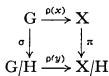
\includegraphics[keepaspectratio]{images/part002_b1d03d5a.jpg}}

于是 \(\pi \circ \rho (x) = \rho (y)\circ \sigma\)，从而

\[
\mathrm{T} _ {x} (\pi) \circ \mathrm{T} _ {e} (\rho (x)) = \mathrm{T} _ {e} (\rho (y)) \circ \mathrm{T} _ {e} (\sigma).
\]

令 \(u \in T_{e}(\mathrm{G/H})\) 满足 \(T_{e}(\rho(y))u = 0\)。存在 \(v \in T_{e}(\mathrm{G})\)，使 \(u = T_{e}(\sigma)v\)。于是 \(T_{x}(\pi)(T_{e}(\rho(x))v) = 0\)，因此 \(T_{e}(\rho(x))v\) 是 Hx 的切向量（Differentiable and Analytic Manifolds, R, 5.10.5），故其具有 \(T_{e}(\rho(x) | H)v'\) 的形式，其中 \(v' \in T_{e}(\mathrm{H})\)。由于 \(T_{e}(\rho(x))\) 是单射，所以 \(v = v'\)，从而 \(v \in T_{e}(\mathrm{H})\)，且 \(u = 0\)。因此 \(T_{e}(\rho(y))\) 是单射。\(T_{e}(\rho(y))\) 的像等于 \(T_{x}(\pi) \circ T_{e}(\rho(x))\) 的像；现在 \(T_{e}(\rho(x))\) 的像在 \(T_{x}(\mathrm{X})\) 中有拓扑补，并且包含 \(T_{x}(\pi)\) 的核。因此可见 \(\rho(y)\) 是浸入，这就完成了 (ii) 的证明。

断言 (iii) 由上述内容和 Differentiable and Analytic Manifolds, R, 5.9.7 得出。

推论。设 G 为李群，H、L 为 G 的正规李子群，且 \(L \subset H\)。则 H/L 是 G/L 的正规李子群，并且从 G/H 到 \((G/L)/(H/L)\) 的典范双射是李群同构。

\subsection{轨道}

命题 14. 设 \(\mathbf{G}\) 为李群，\(\mathbf{X}\) 为解析流形，且 \((g,x)\mapsto gx\) 是 \(\mathbf{G}\) 在 \(\mathbf{X}\) 上的解析左作用律。设 \(x\in \mathbf{X}\)。假设相应的轨道映射 \(\rho (x)\) 是次浸入（如果 \(\mathbf{K}\) 的特征为 0 且 \(\mathbf{X}\) 是有限维的，这总是如此（命题 9 的推论））。令 \(\mathbf{G}_{\mathbf{x}}\) 为稳定子 \(x\) 在 \(\mathbf{G}\) 中的子群。

\begin{enumerate}
\def\labelenumi{(\roman{enumi})}
\item
  \(\mathrm{G}_x\) 是李子群，且 \(\mathrm{T}_e(\mathrm{G}_x) = \mathrm{Ker}\, \mathrm{T}_e(\rho(x))\)。
\item
  齐性空间的典范映射 \(i_x\) 从 \(G / G_x\) 到 \(X\) 是浸入，其像为 \(Gx\)。
\item
  如果进一步轨道 \(\mathbf{G}x\) 是局部闭的且 \(\mathbf{G}\) 的拓扑具有可数基，则 \(\mathbf{G}x\) 是 \(\mathbf{X}\) 的子流形，\(i_x\) 是从流形 \(\mathrm{G} / \mathrm{G}_x\) 到流形 \(\mathbf{G}x\) 的同构，且 \(\mathrm{T}_x(\mathbf{G}x) = \operatorname{Im} \mathrm{T}_e(\rho(x))\)。
\end{enumerate}

\(x\) 在 \(\rho(x)\) 下的逆像是 \(G_x\)。由于 \(\rho(x)\) 是次浸入，\(G_x\) 是子流形，并且对于所有 \(g \in G\)，其切空间 \(J\) 是 \(gG_x = \rho(x)^{-1}(gx)\) 在 \(g\) 处的切空间，且等于 \(\operatorname{Ker} T_g(\rho(x))\)（Differentiable and Analytic Manifolds, R, 5.10.5），从而得到 (i)。令 \(\pi: G \to G/G_x\) 为典范映射。于是 \(i_x \circ \pi = \rho(x)\)。由于 \(G/G_x\) 是 \(G\) 的商流形，这个等式表明 \(i_x\) 是解析的。此外，\(T_g(\rho(x))\) 和 \(T_g(\pi)\) 的核都等于 \(J\)。因此 \(T_{\pi(g)}(i_x)\) 是单射。\(T_{\pi(g)}(i_x)\) 的像等于 \(T_g(\rho(x))\) 的像，因而有拓扑补。这证明了 (ii)。

假设 \(Gx\) 是局部闭的。于是 \(Gx\) 中每一点在 \(Gx\) 中都有一个邻域，它同胚于完备度量空间的闭子空间，因而是 Baire 空间。因此 \(Gx\) 是 Baire 空间（General Topology, Chapter IX, § 5, Proposition 4）。如果 \(G\) 具有可数基，则 \(i_x\) 是从 \(G / G_x\) 到 \(Gx\) 的同胚（General Topology, Chapter IX, § 5）。于是由 (ii) 和 Differentiable and Analytic Manifolds, R, 5.8.3，\(i_x\) 是从流形 \(G / G_x\) 到流形 \(Gx\) 的同构，并且

\[
\mathrm{T} _ {x} (\mathrm{G} x) = \operatorname{Im} \mathrm{T} _ {\pi (e)} (i _ {x}) = \operatorname{Im} \mathrm{T} _ {e} (\rho (x)).
\]

备注。设 G 为有限维李群，X 为 \(C^{r}\) 类流形，且 \((g, x) \mapsto gx\) 是 G 在 X 上的 \(C^{r}\) 类左作用律。则命题 14 仍然成立。唯一需要不同证明的点是 \(G_{x}\) 为李子群这一事实。但若 \(r \neq \omega\)，则 K = R；由于 \(G_{x}\) 显然是闭的，\(G_{x}\) 由§8、定理 2 得出是李子群。

推论。设 G 为拓扑具有可数基的李群，X 为

非空有限维解析流形，且 G 在 X 上有解析左作用律。假设 G 在 X 上传递作用且 K 的特征为 0。则 X 是 G 的李齐性空间。

令 \(x \in X\)。\(x\) 的轨道等于 \(X\)，是闭的，因此可以应用命题 14 (iii)。

\subsection{带算子的向量丛}

设 G 为李群，X 为 \(C^{r}\) 类流形，且 \((g, x) \mapsto gx\) 是 \(C^{r}\) 类的 G 在 X 上的左作用律。设 E 为 \(C^{r}\) 类向量丛，底空间为 X，且 \(\pi: E \to X\) 为 E 到 X 的投影。对于所有 \(x \in X\)，令 \(E_{x}\) 为 E 在 x 处的纤维。令 \((g, u) \mapsto gu\) 为 G 在 E 上的左作用律，使 \(\pi\) 与 G 在 X 和 E 上的作用相容。对于所有 \(g \in G\) 和 \(x \in X\)，将其在 \(E_{x}\) 上的限制 \(u \mapsto gu\) 记为双射 \(\psi_{g,x}\)，它从 \(E_{x}\) 到 \(E_{gx}\)。我们假定，对于所有 \(g \in G\) 和 \(x \in X\)，\(\psi_{g,x}\) 是连续线性的，因而是可赋范空间 \(E_{x}\) 到可赋范空间 \(E_{gx}\) 的同构。

令 \(\phi\) 为自同构 \((g,x)\mapsto (g,gx)\)（定义在流形 \(\mathrm{G}\times \mathrm{X}\) 上）。令 \(p\) 为 \(\mathrm{G}\times \mathrm{X}\) 到 \(\mathbf{X}\) 的典范投影，\(\mathrm{E}'\) 为 \(\mathrm{E}\) 在 \(p\) 下的逆像。令 \(\psi \colon \mathrm{E}'\to \mathrm{E}'\) 为各映射 \(\psi_{g,x}\colon \mathrm{E}_{(g,x)}'\to \mathrm{E}_{(g,gx)}'\) 的和。

定义 4. 如果 \(\psi\) 是向量丛的 \(\phi\)-态射且属于 \(\mathbf{C}^r\) 类，则 \(\mathbf{E}\) 称为向量 \(\mathbf{G}\)-丛，类为 \(\mathbf{C}^r\)。

换言之，E 是 \(C^{r}\) 类向量 G-丛，当且仅当对于所有 \((g_{0}, x_{0}) \in \mathbf{G} \times \mathbf{X}\)，以下条件成立：存在 \((g_{0}, x_{0})\) 在 \(G \times X\) 中的一个开邻域 U，使得，如果 \(E^{\prime} \mid U\)（相应地，\(E^{\prime} \mid \phi(U)\)）借助向量图识别为纤维 M（相应地，N）的平凡向量丛，则映射 \((g, x) \mapsto \psi_{g,x}\) 从 U 到 \(\mathcal{L}(M, N)\) 是 \(C^{r}\) 类的。

映射 \(\psi\) 显然是双射，由上述局部判据可知 \(\psi^{-1}\) 是向量丛的 \(\phi^{-1}\)-态射，因此 \(\psi\) 是向量丛的 \(\phi\)-同构。

以 X 为底空间的平凡向量 G-丛是向量丛 \(X \times F\)（其中 F 是完备可赋范空间），并带有作用律 \((g, (x, f)) \mapsto (gx, f)\) 在 G 的 \(X \times F\) 上的作用。

仍假定定义 4 前的假设和记号，并进一步取 \(\tau\) 为对同构的 \(C^r\) 类向量函子（Differentiable and Analytic Manifolds, R, 7.6.6）。则 \(\tau E\) 是底空间为 \(X\) 的向量丛。对于所有 \(x \in X\)，其纤维 \((\tau E)_x\) 等于 \(\tau (E_x)\)。对于所有可赋范空间 \(N_1, N_2\)，令 \(\operatorname{Isom}(N_1, N_2)\) 表示从 \(N_1\) 到 \(N_2\) 的同构集合。如果 \(g \in G\)，则

\[
\tau (\psi_ {g, x}) \in \operatorname{Isom} ((\tau E) _ {x}, (\tau E) _ {g x}).
\]

\(\tau(\psi_{g,x})\) 定义了左作用律 \((g,u)\mapsto gu\) G 在 \(\tau\) E 上，且 \(\tau\) E 到 X 的典范投影与 G 在 X 和 \(\tau\) E 上的作用相容。

命题 15. 如果 E 是 \(\mathbf{C}^r\) 类向量 G-丛，则 \(\tau \mathbf{E}\) 是 \(\mathbf{C}^r\) 类向量 G-丛。

设 \(g_0, x_0\)、U、M、N 如定义 4 后的段落所述。映射 \((g, x) \mapsto \tau(\psi_{g,x})\) 从 U 到 \(\mathcal{L}(\tau\mathrm{M}, \tau\mathrm{N})\)，是映射 \((g, x) \mapsto \psi_{g,x}\) 从 U 到 \(\mathcal{L}(\mathrm{M}, \mathrm{N})\) 与映射 \(f \mapsto \tau(f)\) 从 \(\operatorname{Isom}(\mathrm{M}, \mathrm{N})\) 到 \(\operatorname{Isom}(\tau\mathrm{M}, \tau\mathrm{N})\) 的复合；这两个映射都是 \(C^r\) 类的，因而复合也如此，从而得到命题。

命题 16. 设 G 为李群，X 为 \(\mathbf{C}^r\) 类流形（\(r \geqslant 2\)），且 \((g, x) \mapsto gx\) 是 G 在 X 上的 \(\mathbf{C}^r\) 类左作用律；因此通过传递结构，G 在 TX 上有一个左作用律。在此作用律下，TX 是 \(\mathbf{C}^{r-1}\) 类向量 G-丛。

令 \(\mathrm{pr}_1\)（相应地，\(\mathrm{pr}_2\)）为从 \(\mathrm{G} \times \mathrm{X}\) 到 \(\mathrm{G}\)（相应地，\(\mathrm{X}\)）的典范投影，并令 \(\mathrm{E}_1\)（相应地，\(\mathrm{E}_2\)）为关于 \(\mathrm{pr}_1\)（相应地，\(\mathrm{pr}_2\)）的 TG（相应地，TX）的逆像。于是向量丛 \(\mathrm{T}(\mathrm{G} \times \mathrm{X})\) 是 \(\mathrm{E}_1\) 和 \(\mathrm{E}_2\) 的直和。令 \(i: \mathrm{E}_2 \to \mathrm{T}(\mathrm{G} \times \mathrm{X})\) 和 \(q: \mathrm{T}(\mathrm{G} \times \mathrm{X}) \to \mathrm{E}_2\) 为由此直和分解定义的典范向量丛态射。令 \(\phi\) 为映射 \((g, x) \mapsto (g, gx)\)，它从 \(\mathrm{G} \times \mathrm{X}\) 到 \(\mathrm{G} \times \mathrm{X}\)。然而，定义 4 中记作 \(\psi\) 的映射（其中取 \(\mathrm{E} = \mathrm{TX}\)）正是 \(q \circ \mathrm{T}(\phi) \circ i\)。但是 \(\mathrm{T}(\phi)\) 是一个 \(\phi\)-态射，并且作为向量丛态射的类为 \(\mathrm{C}^{r-1}\)（Differentiable and Analytic Manifolds, R, 8.1.2）。

推论。若 \(\tau\) 是对同构的 \(\mathbf{C}^r\) 类向量函子，则 \(\tau(\mathrm{TX})\) 是类为 \(\mathbf{C}^{r-1}\) 的向量 G-丛。

这由命题 15 和 16 得出。

注 1. 若 \(\tau\) 是有限维情形下对同构的 \(C^r\) 类向量函子，且 \(E\) 具有有限秩，则 \(\tau E\) 的定义类似，命题 15 仍然成立；只要 \(X\) 是有限维的，命题 16 的推论仍然成立。

例子。取命题 16 的假设和记号，并令 F 为完备可赋范空间。则 \(\mathcal{L}((\mathrm{TX})^p; \mathrm{F})\) 是类为 \(\mathrm{C}^{r-1}\) 的向量 G-丛；如果 K 的特征为零或 X 是有限维的，则 \(\operatorname{Alt}^p(\mathrm{TX}; \mathrm{F})\) 也是如此（参见~Differentiable and Analytic Manifolds, R, 7.7, 7.8）。如果 X 是有限维的，则 \(\bigotimes^p(\mathrm{TX}) \otimes \bigotimes^q(\mathrm{TX})^*\) 是类为 \(\mathrm{C}^{r-1}\) 的向量 G-丛。

命题 17. 设 G 是李群，X 是 G 的左李齐性空间，\(x_0\) 是 X 中的一点，\(G_0\) 是 G 中 \(x_0\) 的稳定子，E 和 E' 是基空间为 X 且类为 \(C^{r}\) 的左向量 G-丛，\(E_0\)（相应地，\(E_0'\)）是 E（相应地，E'）在 \(x_0\) 处的纤维，且 f 是 \(\mathcal{L}(E_0, E_0')\) 中满足 \(f(gu) = g(f(u))\)（对所有 \(u \in E_0\) 和 \(g \in G_0\)）的元素。则存在唯一一个从 E 到 E'、与 G 的作用相容并延拓 f 的态射。这个态射的唯一性是显然的。下面证明其存在性。令 \(g\)、\(g'\) 为 G 中的元素，且 \(u \in E_0\) 满足 \(gu = g'u\)。则 \(g'^{-1}g \in G_0\) 且 \(g'^{-1}gu = u\)，从而 \(g'^{-1}gf(u) = f(u)\)，即 \(gf(u) = g'f(u)\)。因此定义映射 \(\phi\)，其从 E 到 \(E'\)，规定 \(\phi(gu) = gf(u)\)。显然，此映射延拓 \(f\)，并且与 G 的作用相容。我们证明 \(\phi\) 是类为 \(C^r\) 的向量丛态射。令 \(x_1 \in X\)。存在 X 中 \(x_1\) 的开邻域 V 以及 G 的子流形 W，使得映射 \(g \mapsto gx_0\) 是 W 到 V 的同构 \(\theta\)，类为 \(C^r\)。将 V 和 W 缩小后，可设：

\begin{enumerate}
\def\labelenumi{(\arabic{enumi})}
\item
  E \textbar{} V（相应地，E' \textbar{} V）被识别为纤维为 M（相应地，M'）的平凡向量丛；
\item
  若 \(\psi_{g}\)（相应地，\(\psi_{g}^{\prime}\)）表示映射 \(u\mapsto gu\)，其定义域为 \(\mathrm{E}_0\)（相应地，\(\mathrm{E}_0^{\prime}\)），值域为 \(\mathrm{E}_{gx_0}\)（相应地，\(\mathrm{E}_{gx_0}\)），则映射 \(g\mapsto \psi_g\) 和 \(g\mapsto \psi_g^{-1}\)（相应地，\(g\mapsto \psi_g^{\prime}\) 和 \(g\mapsto \psi_g^{\prime -1}\)）从 W 到 \(\mathcal{L}(\mathrm{E}_0,\mathrm{M})\) 和 \(\mathcal{L}(\mathrm{M},\mathrm{E}_0)\)（相应地，\(\mathcal{L}(\mathrm{E}_0',\mathrm{M}')\) 和 \(\mathcal{L}(\mathrm{M}',\mathrm{E}_0'))\)，都是类为 \(C^r\) 的。
\end{enumerate}

对于 \(x \in V\)，令 \(\phi_x: M \to M'\) 为 \(\phi\) 在 \(E_x = M\) 上的限制。于是 \(\phi_x\) 由以下映射复合而成：

\begin{enumerate}
\def\labelenumi{(\arabic{enumi})}
\item
  映射 \((\psi_{\theta^{-1}(x)})^{-1}\)，它从 M 到 \(E_{0}\)；
\item
  从 \(E_{0}\) 到 \(E_{0}'\) 的映射 f；
\item
  映射 \(\psi_{\theta^{-1}(x)}^{\prime}\)，它从 \(\mathbf{E}_0'\) 到 \(\mathbf{M}'\)。
\end{enumerate}

因此可见，映射 \(x \mapsto \phi_x\) 从 V 到 \(\mathcal{L}(\mathbf{M}, \mathbf{M}')\)，且是类为 \(\mathbf{C}^r\) 的。

推论 1. 设 \(\mathrm{E}_0^{\mathbb{G}_0}\) 是 \(\mathrm{E}_0\) 中在 \(\mathbf{G}_0\) 作用下不变的元素所成的集合。对所有 \(u \in \mathrm{E}_0^{\mathbb{G}_0}\)，令 \(\sigma_u\) 为从 X 到 E 的映射，由 \(\sigma_u(gx_0) = gu\)（对所有 \(g \in G\)）定义。

\begin{enumerate}
\def\labelenumi{(\roman{enumi})}
\item
  E 的 G-不变截面†都是类为 \(\mathbf{C}^r\) 的。
\item
  \(u \mapsto \sigma_u\) 是从 \(\mathrm{E}_0^{\mathrm{G}_0}\) 到 E 的 G-不变截面集合的双射。
\end{enumerate}

断言 (ii) 是显然的。为证明 (i)，只需证明每个截面 \(\sigma_{u}\) 都是类为 \(C^r\) 的。令 E' 为基空间 X、纤维为 \(\mathrm{E}_0^{\mathrm{G}_0}\) 的平凡 G-丛。令 \(f\) 为从 \(\mathrm{E}_0^{\mathrm{G}_0}\) 到 \(\mathrm{E}_0\) 的典范嵌入。根据命题 17，存在态射 \(\phi\)，它从 E' 到 E、与 G 的作用相容并延拓 \(f\)。若 \(u \in \mathrm{E}_0^{\mathrm{G}_0}\) 且 \(g \in \mathrm{G}\)，则

\[
\sigma_ {u} (g x _ {0}) = g u = g f (u) = \phi (g u) = \phi ((u, g x _ {0}))
\]

从而有 \(\sigma_u(x) = \phi((u, x))\)，对所有 \(x \in \mathbf{X}\)，这就证明了断言。

*例如，设 G 是有限维实李群，\(G_{0}\) 是 G 的紧李子群，X 是齐性空间 \(G/G_{0}\)。记 X 中 e 的典范像为 \(x_{0}\)。在 \(T_{x_{0}}(X)\) 上存在一个在 \(G_{0}\) 作用下不变的正定对称双线性型（Integration，第 VII 章，第 § 3 节，命题 1）。将上述结果应用于 \((\mathrm{TX})^{*}\otimes(\mathrm{TX})^{*}\)，可见 X 上存在一个在 \(G_{0}\) 作用下不变的解析黎曼度量。

推论 2. 假设 \(G_{0}\) 在 \(E_{0}\) 上平凡作用。令 \(E'\) 为基空间 X、纤维为 \(E_{0}\) 的平凡 G-丛。存在唯一一个从 E 到 \(E'\)、与 G 的作用相容并延拓 \(Id_{E_{0}}\) 的同构。

这立即由命题 17 得出。

注 2. 在本编号中，左作用律处处都可以用右作用律替代。

\subsection{李群的局部定义}

命题 18. 设 \(\mathbf{G}\) 是一个群，\(\mathbf{U}\) 和 \(\mathbf{V}\) 是 \(\mathbf{G}\) 中包含 \(e\) 的两个子集。假设 \(\mathbf{U}\) 具有满足下列条件的解析流形结构：

\begin{enumerate}
\def\labelenumi{(\roman{enumi})}
\item
  \(\mathrm{V} = \mathrm{V}^{-1},\mathrm{V}^2\subset \mathrm{U},\mathrm{V}\) 在 U 中是开集；
\item
  映射 \((x,y)\mapsto xy^{-1}\) 从 \(\mathbf{V}\times \mathbf{V}\) 到 \(\mathbf{U}\)，且是解析的；
\item
  对所有 \(g \in \mathbf{G}\)，存在 \(\mathbf{V}'\)，它是 \(e\) 在 \(\mathbf{V}\) 中的开邻域，使得 \(g\mathbf{V}'g^{-1} \subset \mathbf{U}\)，并且映射 \(x \mapsto gxg^{-1}\) 从 \(\mathbf{V}'\) 到 \(\mathbf{U}\)，且是解析的。
\end{enumerate}

则在 \(\mathbf{G}\) 上存在唯一一个具有下列性质的解析流形结构：

(α) 带此结构的 G 是李群；

(β) V 在 G 中是开集；

\begin{enumerate}
\def\labelenumi{(\Alph{enumi})}
\setcounter{enumi}{24}
\tightlist
\item
  G 和 U 上的流形结构在 V 上诱导出相同的结构。
\end{enumerate}

\begin{enumerate}
\def\labelenumi{(\alph{enumi})}
\item
  令 A 为 V 的开子集，\(v_{0}\) 为 V 中的元素且满足 \(v_{0}A \subset V\)。则 \(v_{0}A\) 是满足 \(v \in V\) 且 \(v_{0}^{-1}v \in A\) 的 v 所成的集合，因而是 V 的开子集（考虑 (ii)）。此外，(ii) 表明，映射 \(v \mapsto v_{0}v\) 从 A 到 \(v_{0}A\)，以及映射 \(v \mapsto v_{0}^{-1}v\) 从 \(v_{0}A\) 到 A，互为解析双射，因而是解析同构。
\item
  取 \(W\)，它是 \(e\) 在 \(V\) 中的开邻域，满足 \(W = W^{-1}\)、\(W^3 \subset V\)，并且存在图表 \((W, \phi, E)\)，它属于流形 \(U\)，其定义域为 \(W\)。对所有 \(g \in G\)，令 \(\phi_g\) 为映射 \(h \mapsto \phi(g^{-1}h)\)，它从 \(gW\) 到 \(E\)。我们证明，图表 \(\phi_g\) 是 \(G\) 的解析相容图表。令 \(g_1, g_2\) 为 \(G\) 中的元素，满足 \(g_1W \cap g_2W \neq \emptyset\)，于是 \(g_2^{-1}g_1\) 和 \(g_1^{-1}g_2\) 属于 \(W^2\)。根据 (a)，\(W \cap g_1^{-1}g_2W\) 是 \(W\) 的开子集，因此
\end{enumerate}

\[
\phi_ {g _ {1}} (g _ {1} \mathrm{W} \cap g _ {2} \mathrm{W}) = \phi (\mathrm{W} \cap g _ {1} ^ {- 1} g _ {2} \mathrm{W})
\]

是 E 的开子集 D。对于 \(d \in \mathbf{D}\)，

\[
\left(\phi_ {g _ {2}} \circ \phi_ {g _ {1}} ^ {- 1}\right) (d) = \phi \left(g _ {2} ^ {- 1} g _ {1} \phi^ {- 1} (d)\right);
\]

由 (a) 可见，\(\phi_{g_2} \circ \phi_{g_1}^{-1}\) 是解析的。

\begin{enumerate}
\def\labelenumi{(\alph{enumi})}
\setcounter{enumi}{2}
\item
  由 (b)，在 \(\mathbf{G}\) 上存在解析流形结构，使 \((\phi_g)_{g\in G}\) 成为 \(\mathbf{G}\) 上的图册。对所有 \(g_0\in \mathbf{G}\)，映射 \(g\mapsto g_0g\)（\(g\in \mathbf{G}\)）保持该图册不变，因而是带此流形结构的 \(\mathbf{G}\) 的自同构。特别地，条件 \((\mathrm{GL}_1)\) 得到满足。
\item
  令 \(v_{0} \in V\)。根据 (ii)，存在 \(A\)，它是 \(e\) 在 \(W\) 中的开邻域，且 \(v_{0}A \subset V\)。这首先证明 \(V\) 是 \(G\) 中的开集。根据 (a)，映射 \(v \mapsto v_{0}v\) 从 \(A\) 到 \(v_{0}A\) 是解析同构，其结构取自 U。根据 (c)，可见 G 和 U 上的流形结构在 \(v_{0}\mathbf{A}\) 上诱导出相同的结构，因而最终在 V 上也相同。
\item
  由 (d)、(ii) 和 (iii)，可见条件 \((\mathrm{GL}_2)\) 和 \((\mathrm{GL}_3)\) 成立。因此 G 是李群。
\item
  如果 G 上的流形结构与 G 的群结构相容，并且 V 是 G 的开子流形，那么 \((\phi_{g})_{g\in G}\) 是 G 上的图册。这就证明了命题的唯一性断言。
\end{enumerate}

命题 19. 设 G 是拓扑群，H 是李群，f 是从群 G 到群 H 的同态。假设存在 G 中 \(e_{G}\) 的一个开邻域、图表 (V, \(\phi\) , E)，它是流形 H 在 \(e_{H}\) 处的图表，以及 E 的一个具有拓扑补空间的闭向量子空间 F，使得 \(f(\mathrm{U}) \subset \mathrm{V}\)，并且 \((\phi \circ f)\mid_U\) 是从 U 到 \(\phi(\mathrm{V}) \cap \mathrm{F}\) 的同胚。则在 G 上存在唯一一个使 f 成为浸入的流形结构；该结构是 H 上流形结构在 f 下的逆像。带此结构的 G 是李群。

由于 G 的平移（相应地，H 的平移）是同胚（相应地，解析同构），f 满足《Differentiable and Analytic Manifolds》R, 5.8.1 中的条件 (R)。于是命题的前两个断言由《Differentiable and Analytic Manifolds》R, 同上处得出。考虑交换图

\[
\begin{array}{c} \mathrm{G} \times \mathrm{G} \xrightarrow {m} \mathrm{G} \\ f \times f \Big \downarrow \qquad \qquad \qquad \qquad \qquad \qquad \qquad \qquad \qquad \Big \downarrow f \\ \mathrm{H} \times \mathrm{H} \xrightarrow {n} \mathrm{H} \end{array}
\]

其中，对于 G（相应地，H）中的 x、y，\(m(x,y)=xy^{-1}\)（相应地，\(n(x,y)=xy^{-1}\)）。则 \(n\circ(f\times f)\) 是解析的，从而 \(f\circ m\) 是解析的；又因为 f 是浸入，所以 m 是解析的。因此 G 是李群。

G 上的李群结构称为 H 上李群结构在 f 下的逆像。

推论。设 G 是拓扑群，N 是 G 的离散正规子群，且 \(\pi\) 是从 G 到 G/N 的典范映射。假设 G/N 上给定了解析流形结构，并且与 G/N 的拓扑群结构相容。则在 G 上存在唯一一个使 \(\pi\) 成为浸入的流形结构；该结构是 G/N 上流形结构在 \(\pi\) 下的逆像。带此结构时，\(\pi\) 是 étale 的，G 是李群，而 G/N 是 G 按 N 作商得到的商李群。

注。设 H 是连通实或复李群，\(\hat{H}\) 是其万有覆盖\(\dagger\)，且 \(\pi\) 是从 \(\hat{H}\) 到 H 的典范映射。当我们把 \(\hat{H}\) 作为李群谈论时，始终指的是 \(\mathbf{H}\) 上的结构在 \(\pi\) 下的逆像结构。

\subsection{李群芽}

定义 5. K 上的李群芽是满足下列条件的系统 (G, e, θ, m)：

\begin{enumerate}
\def\labelenumi{(\roman{enumi})}
\item
  G 是 K 上的解析流形；
\item
  \(e \in G;\)
\item
  \(\theta\) 是从 G 到 G 的解析映射；
\item
  \(m\) 是从开子集 \(\Omega\)（\(\mathbf{G} \times \mathbf{G}\) 的开子集）到 \(\mathbf{G}\) 的解析映射；
\item
  对所有 \(g \in G\)，都有 \((e, g) \in \Omega\)、\((g, e) \in \Omega\) 以及 \(m(e, g) = m(g, e) = g\)；
\end{enumerate}

\[
g \in G, (g, \theta (g)) \in \Omega , (\theta (g), g) \in \Omega , m (g, \theta (g)) = m (\theta (g), g) = e;
\]

\begin{enumerate}
\def\labelenumi{(\roman{enumi})}
\setcounter{enumi}{6}
\tightlist
\item
  若 \(g, h, k\) 是 \(G\) 中满足 \((g, h) \in \Omega\)、\((h, k) \in \Omega\)、\((m(g, h), k) \in \Omega\) 和 \((g, m(h, k)) \in \Omega\) 的元素，则 \(m(m(g, h), k) = m(g, m(h, k))\)。
\end{enumerate}

e 称为李群芽的单位元。我们通常用 gh 代替 \(m(g, h)\)，并且（滥用记号）用 \(g^{-1}\) 代替 \(\theta(g)\)。

李群 G 是取 \(e, \theta, m\) 为显然选择的李群芽。设 G 是李群芽。则 \(ee^{-1} = e\)，即

\[
e ^ {- 1} = e.\tag{8}
\]

对所有 \(g\in G\)

\[
g = e g = ((g ^ {- 1}) ^ {- 1} g ^ {- 1}) g = (g ^ {- 1}) ^ {- 1} (g ^ {- 1} g) = (g ^ {- 1}) ^ {- 1} e,
\]

即

\[
(g ^ {- 1}) ^ {- 1} = g.\tag{9}
\]

G 的一个子集若在映射 \(g \mapsto g^{-1}\) 下不变，就称为对称的。流形 G 取点 e、映射 \(g \mapsto g^{-1}\) 以及映射 \((g, h) \mapsto hg\)，构成称为 G 的对立李群芽的李群芽 G \(^{\nu}\)。

若对于所有 \((g,h)\in \mathbf{G}\times \mathbf{G}\) 中满足 \(gh\) 有定义的元素，\(hg\) 也有定义且等于 \(gh\)，则称李群芽 G 为交换的。

设 \(G\) 是李群芽。由 \((g, h) \in G \times G\) 且 \(gh\) 有定义的元素所成的集合是 \((e, e)\) 的邻域。另一方面，映射 \((g, h) \mapsto gh\) 和 \(g \mapsto g^{-1}\) 是连续的。因此 \((gh)k = g(hk)\)，其中 \(g, h, k\) 充分接近 \(e\)。同样，\((h^{-1}g^{-1})(gh) = h^{-1}(eh) = h^{-1}h = e\)，其中 \(g, h\) 充分接近 \(e\)，于是右乘 \((gh)^{-1}\)，

\begin{enumerate}
\def\labelenumi{(\arabic{enumi})}
\setcounter{enumi}{9}
\tightlist
\item
\end{enumerate}

\((gh)^{-1} = h^{-1}g^{-1}\)，其中 \(g,h\) 充分接近 \(e\)。

命题 20. 设 G 是李群芽且 \(g \in G\)。存在 e 的开邻域 U 和 g 的开邻域 V，具有下列性质：

\begin{enumerate}
\def\labelenumi{(\alph{enumi})}
\item
  对所有 \(u \in U\)，ug 有定义；
\item
  \(vg^{-1}\) 对所有 \(v \in V\) 都有定义；
\item
  映射 \(u \mapsto ug\)、\(v \mapsto vg^{-1}\) 彼此互为从 U 到 V 及从 V 到 U 的解析同构。
\end{enumerate}

  由于乘积的定义域是 \(\mathbf{G} \times \mathbf{G}\) 中的开集，存在 \(e\) 的开邻域 U 和 \(g\) 的开邻域 V，具有性质 (a) 和 (b)。令 \(\eta(u) = ug\)（\(u \in \mathrm{U}\)），\(\eta'(v) = vg^{-1}\)（\(v \in \mathrm{V}\)）。缩小 U 和 V，可设 \((ug)g^{-1} = u\) 以及 \((vg^{-1})g = v\)，其中 \(u \in \mathrm{U}\) 和 \(v \in \mathrm{V}\)。于是 \(\eta\) 和 \(\eta'\) 是单射。再缩小 U，可设 \(\eta(\mathrm{U}) \subset \mathrm{V}\)。于是 \(\eta'(\mathrm{V}) \supset \mathrm{U}\)，且 \(\eta(\mathrm{U})\) 是 \(\eta'\) 下 U 的逆像，因而是 V 中 \(g\) 的开邻域。将 V 替换为 \(\eta(\mathrm{U})\)，最终得到 \(\eta\) 和 \(\eta'\) 是解析的互逆双射。

设 \(G_{1}, G_{2}\) 是两个李群芽，单位元分别为 \(e_{1}, e_{2}\)。从 \(G_{1}\) 到 \(G_{2}\) 的映射 f 若满足下列条件，就称为态射：

\begin{enumerate}
\def\labelenumi{(\roman{enumi})}
\item
  \(f\) 是解析的；
\item
  \(f(e_{1}) = e_{2};\)
\item
  若 \(g, h\) 是 \(\mathbf{G}_1\) 中满足 \(gh\) 有定义的元素，则 \(f(g)f(h)\) 有定义且等于 \(f(gh)\)。
\end{enumerate}

令 \(g \in G_1\)。由于 \(gg^{-1}\) 有定义且等于 \(e_1, f(g)f(g^{-1})\) 有定义并等于 \(e_2\)，从而

\[
f (g) ^ {- 1} = f (g) ^ {- 1} \left(f (g) f \left(g ^ {- 1}\right)\right) = \left(f (g) ^ {- 1} f (g)\right) f \left(g ^ {- 1}\right)
\]

即

\[
f (g) ^ {- 1} = f (g ^ {- 1}).\tag{11}
\]

两个态射的复合仍是态射。

若 \(f: \mathbf{G}_1 \to \mathbf{G}_2\) 和 \(f': \mathbf{G}_2 \to \mathbf{G}_1\) 互为逆态射，则它们是同构（特别使用公式 (11)）。

设 \(G_{1}\)、\(G_{2}\) 是两个李群芽，f 是从 \(G_{1}\) 到 \(G_{2}\) 的映射，满足上述条件 (ii) 和 (iii)，并且在 \(e_{1}\) 的一个开邻域内解析。利用命题 20，可仿照命题 4 证明 f 是态射。

设 \((\mathbf{G}, e, \theta, m)\) 是李群芽，\(\Omega\) 是 \(m\) 的定义集。令 \(\mathbf{H}\) 为 \(\mathbf{G}\) 的子流形，它包含 \(e\) 且在 \(\theta\) 下稳定。假设集合 \(\Omega_1\)（由 \((x, y) \in \Omega \cap (\mathbf{H} \times \mathbf{H})\) 中满足 \(m(x, y) \in \mathbf{H}\) 的元素所成）在 \(\mathbf{H} \times \mathbf{H}\) 中是开集。则 \((\mathbf{H}, e, \theta | \mathbf{H}, m | \Omega_1)\) 是李群芽。这样的李群芽称为 \(\mathbf{G}\) 的李子群芽。将 \(\mathbf{H}\) 典范嵌入 \(\mathbf{G}\) 的映射是态射。若 \(f: \mathbf{L} \to \mathbf{G}\) 是李群芽的态射且 \(f(\mathbf{L}) \subset \mathbf{H}\)，则 \(f: \mathbf{L} \to \mathbf{H}\) 是李群芽的态射。

设 K 的特征为 0。若将 H 是 G 的子流形这一假设替换为 H 是 G 的拟子流形这一假设，上述段落的结果仍然成立（参见《Differentiable and Analytic Manifolds》R, 5.8.5）。此时 H 称为 G 的李拟子群芽。

若 G 是单位元为 e 的李群芽，则 G 中 e 的每个对称开邻域都是 G 的李子群芽。（当 G 是李群时尤其如此。）设 H 是 G 的李子群芽；若 H 是 G 中 e 的邻域，则根据命题 20，H 在 G 中是开集。

有限个李群芽的乘积李群芽按显然的方式定义。

命题 21. 设 G、H 是两个李群芽，\(\phi\) 是从 G 到 H 的态射。下列条件等价：

\begin{enumerate}
\def\labelenumi{(\roman{enumi})}
\item
  \(\phi\) 在 \(e\) 处是 étale 的；
\item
  存在 G、H 的开李子群芽 G'、H'，使得 \(\phi|G'\) 是从 G' 到 H' 的同构。
\end{enumerate}

蕴含 \(\langle \mathrm{ii}\rangle \Rightarrow \langle \mathrm{i}\rangle\) 是显然的。假设 \(\phi\) 在 \(e\) 处是 étale 的。存在开李子群芽 \(\mathbf{G}_1\)，它是 \(\mathbf{G}\) 的开李子群芽，使得 \(\phi (\mathbf{G}_1)\) 在 \(\mathbf{H}\) 中是开集，并且 \(\phi |\mathbf{G}_1\) 是流形 \(\mathbf{G}_1\) 到流形 \(\phi (\mathbf{G}_1)\) 的同构。于是存在开李子群芽 \(\mathbf{G}'\)，它是 \(\mathbf{G}_1\) 的开李子群芽，使得 \(\mathbf{G}\) 中 \(\mathbf{G}'\) 的两个元素的乘积总有定义且属于 \(\mathbf{G}_1\)。若 \(g, g'\) 是 \(\mathbf{G}'\) 中满足 \(\mathrm{gg}^{\prime}\in \mathrm{G}'\) 的元素，则 \(\phi (g)\phi (g') = \phi (gg')\in \phi (\mathbf{G}')\)；若 \(g, g'\) 是 \(\mathbf{G}'\) 中满足 \(gg^{\prime}\in G_1 - G'\) 的元素，则

\[
\phi (g) \phi (g ^ {\prime}) = \phi (g g ^ {\prime}) \in \phi (\mathrm{G} _ {1}) - \phi (\mathrm{G} ^ {\prime}).
\]

因此 \(\phi |G^{\prime}\) 是李群芽 \(G^{\prime}\) 到 H 的开李子群芽 \(\phi (G^{\prime})\) 的同构。

若命题 21 的条件成立，则称 G 和 H 局部同构。

命题 22. 设 H 是李群，U 是 H 的李子群芽，N 是由 \(g \in \mathrm{H}\) 所成的集合，其中 U 与 \(g\mathrm{Ug}^{-1}\) 在 \(e\) 处具有相同的芽（《General Topology》，第 I 章，第 § 6 节，编号 10）。则 \(N\) 是包含 U 的 H 的子群。在 \(\mathbb{N}\) 上存在唯一一个具有下列性质的解析流形结构：

\begin{enumerate}
\def\labelenumi{(\roman{enumi})}
\item
  带此结构的 N 是李群；
\item
  U 是 N 的开子流形；
\item
  从 \(\mathbf{N}\) 到 \(\mathbf{H}\) 的典范嵌入是浸入。
\end{enumerate}

显然，\(\mathbf{N}\) 是 \(\mathbf{H}\) 的子群。若 \(g \in \mathbf{U}\)，则 \(ge \in \mathbf{U}\) 且 \(geg^{-1} \in \mathbf{U}\)，因而 \(gu \in \mathbf{U}\) 且 \(gug^{-1} \in \mathbf{U}\)，其中 \(u\) 充分接近 \(e\)（在 \(\mathbf{U}\) 中），所以 \(g\mathrm{U}g^{-1}\) 在 \(e\) 处的芽包含于 \(\mathbf{U}\) 的芽；交换 \(g\) 和 \(g^{-1}\) 后，可见 \(g\mathrm{U}g^{-1}\) 和 \(\mathbf{U}\) 在 \(e\) 处的芽相等。因此 \(\mathbf{U} \subset \mathbf{N}\)。

令 \(\mathbf{V}\) 为 \(e\) 在 \(\mathbf{U}\) 中的开邻域，使 \(\mathrm{V} = \mathrm{V}^{-1}\)、\(\mathrm{V}^2 \subset \mathrm{U}\)。第 9 号命题 18 的条件 (i)、(ii)、(iii)（其中以 \(\mathrm{G}\) 替换为 \(\mathrm{N}\)）成立。于是，在 \(\mathbf{N}\) 上存在解析流形结构，具有下列性质：\((\alpha)\) 带此结构的 \(\mathbf{N}\) 是李群；\((\beta)\) \(\mathbf{V}\) 在 \(\mathbf{N}\) 中是开集；\((\gamma)\) \(\mathbf{N}\) 和 \(\mathbf{U}\) 上的流形结构在 \(\mathbf{V}\) 上诱导出相同的结构。由于 \(\mathbf{V}\) 是 \(\mathbf{H}\) 的子流形，从 \(\mathbf{N}\) 到 \(\mathbf{H}\) 的典范嵌入在 \(e\) 处是浸入，因而在 \(\mathbf{N}\) 的每一点处都是浸入。令 \(u \in \mathbf{U}\)。存在 \(V'\)，它是 e 在 V 中的开邻域，使映射 \(v \mapsto vu\) 在 \(V'\) 上是解析同构，映到 U 中 u 的一个开邻域（命题 20），同时也映到 N 中 u 的一个开邻域。因此 U 在 N 中是开集，并且 U 的恒等映射关于 U 上给定的流形结构和 N 上的开子流形结构是同构；换言之，U 是 N 的开子流形。

最后，考虑 N 上具有命题条件 (i)、(ii) 的解析流形结构，并令 \(N^{*}\) 为由此得到的李群。于是从 N 到 \(N^{*}\) 的恒等映射在 e 处是 étale 的，因而是李群同构。这证明了命题的唯一性断言。

设 H 是李群，U 是 H 的李拟子群芽，N 是由 \(g \in H\) 所成的集合，其中 U 与 \(gUg^{-1}\) 在 e 处具有相同芽。若 K 的特征为 0，则在 G 上存在唯一一个具有命题 22 的条件 (i)、(ii) 的流形结构。证明与命题 22 相同。

推论。沿用命题 22 的记号，令 G 为 H 中由 U 生成的子群。则 G 是 N 的开子群。在 G 上存在唯一一个李群结构，使 U 是 G 的开子流形，且从 G 到 H 的典范嵌入是浸入。

注。沿用命题 22 及其推论的记号，假设 K 的特征为 0，H 是有限维的，且 U 上的拓扑具有可数基。即使有这些假设，也可能 G 在 H 中不是闭集（习题 3）。但是，若 G 是闭集，则 G 是 H 的李子群。因为映射 \((g,h)\mapsto gh\) 是 G 在 H 上的解析左作用律，e 的轨道是 G。于是我们的断言由命题 2 (iv) 和命题 14 (iii) 得出。

\subsection{作用律片段}

设 \((G, e, \theta, m)\) 是李群芽，X 是类为 \(C^r\) 的流形。

定义 6. 类为 \(\mathbf{C}^r\) 的 \(\mathbf{G}\) 在 \(\mathbf{X}\) 上的左作用律片段，是一个映射 \(\psi\)，定义在 \(\Omega\) 上；该开集位于 \(\mathbf{G} \times \mathbf{X}\) 中，包含 \(\{e\} \times \mathbf{X}\)，且该映射取值于 \(\mathbf{X}\)，并具有下列性质：

\begin{enumerate}
\def\labelenumi{(\roman{enumi})}
\item
  \(\psi\) 是类为 \(C^{r}\) 的；
\item
  对所有 \(x \in X\)，\(\psi(e, x) = x\)；
\item
  存在一个邻域 \(\Omega_1\)，它是 \(\{e\} \times \{e\} \times \mathbf{X}\) 在 \(\mathbf{G} \times \mathbf{G} \times \mathbf{X}\) 中的邻域，使得对于 \((g, g', x) \in \Omega_1\)，\(m(g, g')\)、\(\psi(m(g, g'), x)\) 和 \(\psi(g, \psi(g', x))\) 都有定义，并且 \(\psi(g, \psi(g', x)) = \psi(m(g, g'), x)\)。
\end{enumerate}

类为 \(\mathbf{C}^r\) 的右作用律片段类似定义。

我们通常用 \(gx\) 代替 \(\psi(g, x)\)。

设 \(G'\) 是 G 的李子群芽，\(X'\) 是 X 的子流形。假设集合 \(\Omega'\)，即由 \((g,x)\in \Omega \cap (\mathrm{G}'\times \mathrm{X}')\) 中满足 \(\psi (g,x)\in \mathrm{X}'\) 的元素组成的集合，在 \(\mathrm{G}'\times \mathrm{X}'\) 中是开集（若 \(\mathbf{X}'\) 在 \(\mathbf{X}\) 中是开集，则这一条件总能满足）。则 \(\psi |\Omega '\) 是类为 \(\mathrm{C}^r\) 的左作用律片段，作用于 \(\mathrm{G}'\) 和 \(\mathrm{X}'\)，称为由 \(\psi\) 限制到 \(\mathrm{G}'\) 和 \(\mathrm{X}'\) 所得到的作用律片段。

命题 23. 设 \((\mathbf{G}, e, \theta, m)\) 是李群芽，\(\mathbf{X}\) 是类为 \(\mathbf{C}^r\) 的流形，\(x_0\) 是 \(\mathbf{X}\) 中的一点，\(\Omega\) 是 \((e, x_0)\) 在 \(\mathbf{G} \times \mathbf{X}\) 中的开邻域，\(\psi\) 是从 \(\Omega\) 到 \(\mathbf{X}\) 的映射，具有下列性质：

\begin{enumerate}
\def\labelenumi{(\roman{enumi})}
\item
  \(\psi\) 是类为 \(C^{r}\) 的；
\item
  \(\psi(e, x)\) 在 x 充分接近 \(x_{0}\) 时等于 x；
\item
  \(\psi(m(g, g'), x) = \psi(g, \psi(g', x))\)，其中 \((g, g', x)\) 充分接近 \((e, e, x_0)\)。
\end{enumerate}

则存在开邻域 \(\mathbf{X}'\)，它是 \(x_0\) 在 \(\mathbf{X}\) 中的开邻域，以及开子集 \(\Omega'\)，它是 \(\Omega \cap (\mathrm{G} \times \mathrm{X}')\) 的开子集，使得 \(\psi|\Omega'\) 是类为 \(\mathbf{C}^r\) 的左作用律片段，作用于 \(\mathbf{G}\) 和 \(\mathbf{X}'\)。

存在开邻域 \(\mathbf{X}'\)，它是 \(x_0\) 在 \(\mathbf{X}\) 中的开邻域，以及开邻域 \(\mathbf{G}'\)，它是 \(e\) 在 \(\mathbf{G}\) 中的开邻域，使得 \(\psi(e, x) = x\) 对所有 \(x \in \mathbf{X}'\) 成立，并且

\[
\psi (g, \psi (g ^ {\prime}, x)) = \psi (m (g, g ^ {\prime}), x)
\]

对于 \((g, g', x) \in \mathrm{G}' \times \mathrm{G}' \times \mathrm{X}'\)。令 \(\Omega'\) 为由 \((g, x) \in \Omega \cap (\mathrm{G}' \times \mathrm{X}')\) 中满足 \(\psi(g, x) \in \mathrm{X}'\) 的元素所成的集合。于是 \(\Omega'\) 在 \(\mathrm{G} \times \mathrm{X}'\) 中是开集，并且 \(\mathrm{X}'\)、\(\Omega'\) 具有命题中的性质。

引理 3. 设 \(\mathbf{X}\) 是正规空间，\((\mathbf{X}_i)_{i\in I}\) 是 \(\mathbf{X}\) 的局部有限开覆盖。对所有 \((i,j)\in I\times I\) 以及所有 \(x\in \mathbf{X}_i\cap \mathbf{X}_j\)，令 \(\mathrm{V}_{ij}(x)\) 为一个 \(x\) 的邻域，包含于 \(\mathbf{X}_i\cap \mathbf{X}_j\)。于是可以为每个 \(x\in X\) 关联 \(\mathrm{V}(x)\)，它是 \(x\) 的一个邻域，使下列条件成立：

\begin{enumerate}
\def\labelenumi{(\alph{enumi})}
\item
  若 \(x \in \mathbf{X}_i \cap \mathbf{X}_j\)，则 \(\mathrm{V}(x) \subset \mathrm{V}_{ij}(x)\)；
\item
  若 \(\mathrm{V}(x)\) 与 \(\mathrm{V}(y)\) 相交，则存在 \(i\in \mathbf{I}\)，使 \(\mathrm{V}(x)\cup \mathrm{V}(y)\subset \mathrm{X}_i\)
\end{enumerate}

存在开覆盖 \(\langle \mathrm{X}_i\rangle_{i\in I}\)，它覆盖 \(\mathbf{X}\)，使得 \(\overline{\mathbf{X}}_i' \subset \mathbf{X}_i\) 对所有 \(i \in I\) 成立（《General Topology》，第 IX 章，第 § 4 节，定理 3）。令 \(x \in \mathbf{X}\)。令 \(\mathrm{V}_1(x)\) 为 \(\mathrm{V}_{ij}(x)\) 与 \(\mathbf{X}_k'\) 的交集，其中这些集合包含 \(x\)；这是 \(x\) 的开邻域。令 \(\mathrm{V}_2(x)\) 为 \(x\) 的一个邻域，包含于 \(\mathrm{V}_1(x)\) 且只与有限个 \(\mathbf{X}_i\) 相交。于是 \(\mathrm{V}_2(x)\) 只与有限个 \(\overline{\mathbf{X}}_i'\) 相交，因此下式中的集合

\[
\mathrm{V} (x) = \mathrm{V} _ {2} (x) \cap \bigcap_ {i \in I, x \notin \overline {{\mathrm{X}}} _ {i} ^ {\prime}} (\mathrm{X} - \overline {{\mathrm{X}}} _ {i} ^ {\prime})
\]

是 \(x\) 的邻域。若 \(x \in \mathrm{X}_1 \cap \mathrm{X}_j\)，则 \(\mathrm{V}_1(x) \subset \mathrm{X}_1 \cap \mathrm{X}_j\)，从而 \(\mathrm{V}(x) \subset \mathrm{X}_1 \cap \mathrm{X}_j\)。令 \(x, y\) 属于 \(\mathrm{X}\)，并假设 \(\mathrm{V}(x)\) 与 \(\mathrm{V}(y)\) 相交。存在 \(i \in I\)，使 \(x \in \mathrm{X}_i'\)。于是 \(\mathrm{V}_1(x) \subset \mathrm{X}_i'\)，从而 \(\mathrm{V}(x) \subset \mathrm{X}_i'\)，并且 \(\mathrm{V}(y) \cap \overline{\mathrm{X}_i'} \neq 0\)。于是 \(y \in \overline{\mathrm{X}_i'}\)，根据 \(\mathrm{V}(y)\) 的定义，从而 \(y \in \mathrm{X}_i\) 且 \(\mathrm{V}(y) \subset \mathrm{X}_i\)。因此 \(\mathrm{X}_i\) 包含 \(\mathrm{V}(x)\) 和 \(\mathrm{V}(y)\)。

命题 24. 设 G 是李群芽，X 是类为 \(C^{r}\) 的流形，且 (X \(_{i}\) ) \(_{i \in I}\) 是 X 的局部有限开覆盖。对所有 i ∈ I，令 \(\psi_{i}\) 为 G 上类为 \(C^{r}\) 的左作用律片段，作用于 X \(_{i}\)。假设 X 的底层拓扑空间是正规空间，并且对于所有 (i, j) ∈ I × I 以及所有 x ∈ X \(_{i}\) ∩ X \(_{j}\)，\(\psi_{i}\) 与 \(\psi_{j}\) 在 (e, x) 的一个邻域上重合。存在左作用律片段 \(\psi\)，它是 G 在 X 上的类为 \(C^{r}\) 的左作用律片段，使得对所有 i ∈ I 以及所有 x ∈ X \(_{i}\)，\(\psi_{i}\) 与 \(\psi\) 在 (e, x) 的一个邻域上重合。

对所有 \((i,j)\in \mathrm{I}\times \mathrm{I}\) 以及所有 \(x\in \mathrm{X}_i\cap \mathrm{X}_j\)，选取 \(\mathrm{V}_{ij}(x)\)，它是 \(x\) 的开邻域且包含于 \(\mathrm{X}_i\cap \mathrm{X}_j\)，使 \(\psi_i\) 和 \(\psi_j\) 在 \(\{e\} \times \mathrm{V}_{ij}(x)\) 在 \(\mathrm{G}\times \mathrm{X}\) 中的一个邻域上有定义且相等。对所有 \(x\in \mathrm{X}\)，选取 \(\mathrm{V}(x)\)，它是 \(x\) 在 \(\mathrm{X}\) 中的开邻域，使引理 3 的条件 (a) 和 (b) 得到满足。令 \(\mathbf{I}_x\) 为由 \(i\in \mathrm{I}\) 且 \(x\in \mathrm{X}_i\) 的 i 所成的集合。这是有限集。令 \(\mathrm{U}_x\) 为由 \((g,y)\in \mathrm{G}\times \mathrm{V}(x)\) 所成的集合，其中 \(\psi_i\)（\(i\in \mathrm{I}_x\)）在 \((g,y)\) 的一个邻域上有定义且彼此重合。于是 \(\mathrm{U}_x\) 是开集且 \((e,x)\in \mathrm{U}_x\)。对于 \(\psi_i\)（\(i\in \mathrm{I}_x\)），它们在 \(\mathrm{U}_x\) 上都有相同的限制。令 \(x,y\) 属于 \(\mathrm{X}\)。若 \(\mathrm{U}_x\) 与 \(\mathrm{U}_y\) 相交，则 \(\mathrm{V}(x)\) 与 \(\mathrm{V}(y)\) 相交，因而存在 \(i\in \mathrm{I}\) 使

\[
\mathrm{V} (x) \cup \mathrm{V} (y) \subset \mathrm{X} _ {i}.
\]

于是 \(i \in \mathrm{I}_x, i \in \mathrm{I}_y, \psi_i | \mathrm{U}_x = \psi_x, \psi_i | \mathrm{U}_y = \psi_y\)，从而

\[
\psi_ {x} | (\mathrm{U} _ {x} \cap \mathrm{U} _ {y}) = \psi_ {y} | (\mathrm{U} _ {x} \cap \mathrm{U} _ {y}).
\]

因此，\(\psi_x\) 定义了映射 \(\psi\)，它从 \(\mathbf{U} = \bigcup_{x\in \mathbf{X}}\mathbf{U}_x\) 到 \(\mathbf{X}\)，且 \(\mathbf{U}\) 是 \(\{e\} \times \mathbf{X}\) 在 \(\mathbf{G}\times \mathbf{X}\) 中的开邻域。显然，\(\psi\) 是类为 \(C^r\) 的，且 \(\psi (e,x) = x\) 对所有 \(x\in \mathbf{X}\) 成立。对于所有 \(i\in \mathbf{I}\) 及所有 \(x\in \mathrm{X}_i\)，\(\psi\) 与 \(\psi_x\) 及 \(\psi_i\) 在 \((e,x)\) 的一个邻域上重合，于是 \(\psi\) 满足定义 6 的条件 (iii)。

\section{李群的切向量群}

\subsection{切向复合律}

设 X 和 Y 是类为 \(C^{r}\) 的流形。我们知道（《Differentiable and Analytic Manifolds》R, 8.1.4），\(X \times Y\) 是类为 \(C^{r}\) 的流形，并且映射 \((\mathrm{T}(\mathrm{pr}_{1}), \mathrm{T}(\mathrm{pr}_{2}))\)，即到典范投影的切映射之积，是类为 \(C^{r-1}\) 的同构，从 \(\mathrm{T}(\mathrm{X} \times \mathrm{Y})\) 到 \(\mathrm{T}(\mathrm{X}) \times \mathrm{T}(\mathrm{Y})\)。这个同构与基空间为 \(X \times Y\) 的向量丛结构相容，并允许我们将 \(\mathrm{T}(\mathrm{X} \times \mathrm{Y})\) 识别为 \(\mathrm{T}(\mathrm{X}) \times \mathrm{T}(\mathrm{Y})\)。令 \(a \in \mathbf{X}, b \in \mathbf{Y}, u \in \mathrm{T}_a(\mathbf{X}), v \in \mathrm{T}_b(\mathbf{Y})\)；上述识别使我们可以把 \((u, v)\) 视为 \(\mathrm{T}_{(a,b)}(\mathbf{X} \times \mathbf{Y})\) 中的元素；于是

\[
(u, v) = (u, 0) + (0, v)
\]

并且 \((u,0)\)（相应地，\((0,v))\) 是 \(u\)（相应地，\(v\)）在浸入 \(x\mapsto (x,b)\)（相应地，\(y\mapsto (a,y)\)）的切映射下的像，该浸入将 X（相应地，Y）映入 \(\mathbf{X}\times \mathbf{Y}\)。需要精确说明时，我们将 \(0_{a}\) 记为 \(\mathrm{T}_a(X)\) 的零元素。

现在设 X、Y、Z 是类为 \(C^{r}\) 的流形，且 f 是类为 \(C^{r}\) 的从 \(X \times Y\) 到 Z 的映射。利用上述识别，切映射是类为 \(C^{r-1}\) 的从 \(T(X) \times T(Y)\) 到 \(T(Z)\) 的映射。对于 \(u \in T_{a}(X)\) 和 \(v \in T_{b}(Y)\)，

\begin{enumerate}
\def\labelenumi{(\arabic{enumi})}
\tightlist
\item
\end{enumerate}

\[
\mathrm{T} (f) (u, v) = \mathrm{T} (f) (u, 0 _ {b}) + \mathrm{T} (f) (0 _ {a}, v),
\]

\[
\mathrm{T} (f) \left(0 _ {a}, 0 _ {b}\right) = 0 _ {f (a, b)}.\tag{2}
\]

另一方面，映射 \(y \mapsto f(a, y)\) 是浸入 \(y \mapsto (a, y)\) 与 f 的复合；因此

\begin{enumerate}
\def\labelenumi{(\arabic{enumi})}
\setcounter{enumi}{2}
\item
  \(\mathrm{T}(f)(0,v)\) 是 v 在切映射 \(y\mapsto f(a,y)\) 下的像。同样，
\item
  \(\mathbf{T}(f)(u,0)\) 是 \(u\) 在切映射 \(x\mapsto f(x,b)\) 下的像。
\end{enumerate}

若映射 \(f\) 从 \(\mathbf{X} \times \mathbf{Y}\) 到 \(\mathbf{Z}\) 记作 \((x, y) \mapsto xy\)，则常用 \(uv\) 表示元素 \(T(f)(u, v)\)，其中 \(u \in T(\mathbf{X})\)、\(v \in T(\mathbf{Y})\)。

设 X 是类为 \(C^{r}\) 的流形，且有复合律 \(m: X \times X \to X\)，其类为 \(C^{r}\)。则 \(T(m)\) 是类为 \(C^{r-1}\) 的 \(T(X)\) 上的复合律。它称为与 m 相切的复合律。从 \(T(X)\) 投影到 X 的典范投影 p 与复合律 m 和 \(T(m)\) 相容；换言之，

\[
p \circ \mathrm{T} (m) = m \circ (p \times p).\tag{5}
\]

由 (2) 可得

\[
\mathrm{T} (m) \left(0 _ {x}, 0 _ {y}\right) = 0 _ {m (x, y)}\tag{6}
\]

对所有 \(x, y\) 属于 \(\mathbf{X}\)，换言之，零截面 \(x \mapsto 0_x\)（属于 \(\mathrm{T}(\mathbf{X})\)）与律 \(m\) 和 \(\mathrm{T}(m)\) 相容。

命题 1. 设 X 是类为 \(\mathbf{C}^r\) 的流形，且 \(m\) 是 X 上类为 \(\mathbf{C}^r\) 的复合律。若 \(m\) 是结合的（相应地，交换的），则 \(\mathrm{T}(m)\) 是结合的（相应地，交换的）。

若 \(m\) 是结合的，则 \(m \circ (m \times \mathrm{Id}_{\mathbf{x}}) = m \circ (\mathrm{Id}_{\mathbf{x}} \times m)\)，从而

\[
\mathrm{T} (m) \circ (\mathrm{T} (m) \times \mathrm{Id} _ {\mathrm{T} (\mathbf {X})}) = \mathrm{T} (m) \circ (\mathrm{Id} _ {\mathrm{T} (\mathbf {X})} \times \mathrm{T} (m))
\]

从而 \(\mathrm{T}(m)\) 是结合的。令 \(s\) 为映射 \((x,y)\mapsto (y,x)\)，它从 \(\mathbf{X}\times \mathbf{X}\) 到 \(\mathbf{X}\times \mathbf{X}\)。若 \(m\) 是交换的，则 \(m\circ s = m\)，从而

\[
\mathrm{T} (m) \circ \mathrm{T} (s) = \mathrm{T} (m).
\]

但是，\(\mathrm{T}(s)\) 是映射 \((u,v)\mapsto (v,u)\)，它从 \(\mathrm{T}(\mathbf{X})\times \mathrm{T}(\mathbf{X})\) 到 \(\mathrm{T}(\mathbf{X})\times \mathrm{T}(\mathbf{X})\)。因此 \(\mathrm{T}(m)\) 是交换的。

命题 2. 设 X 是类为 \(\mathbf{C}^r\) 的流形，\(m\) 是 X 上类为 \(\mathbf{C}^r\) 的复合律，\(e\) 是 \(m\) 的单位元。

\begin{enumerate}
\def\labelenumi{(\roman{enumi})}
\item
  向量 \(0_{e}\) 是 \(\mathbf{T}(m)\) 的单位元。
\item
  \(\mathrm{T}_{e}(\mathbf{X})\) 在 \(\mathrm{T}(m)\) 下稳定，并且 \(\mathrm{T}_{e}(\mathbf{X})\) 上由 \(\mathrm{T}(m)\) 诱导的复合律是 \(\mathrm{T}_{e}(\mathbf{X})\) 上的向量空间加法。
\item
  令 U 为 X 的开子集，\(\alpha\) 为从 U 到 X 的类为 \(C^{r}\) 的映射，使得对所有 \(x \in U\)，\(\alpha(x)\) 是 x 在 m 下的逆元。则对所有 \(u \in T(U)\)，\(T(\alpha)u\) 是 u 在 \(T(m)\) 下的逆元。
\end{enumerate}

性质 (3) 和 (4) 表明，\(\mathrm{T}(m)(0_e,u) = \mathrm{T}(m)(u,0_e) = u\) 对所有 \(u\in \mathrm{T}(\mathbf{X})\) 成立，从而得到 (i)。对于 \(u,v\)，它们属于 \(\mathrm{T}_e(\mathbf{X})\)，

\[
\mathrm{T} (m) (u, v) = \mathrm{T} (m) (u, 0 _ {e}) + \mathrm{T} (m) (0 _ {e}, v) = u + v,
\]

从而得到 (ii)。最后，关系 \(m(x, \alpha(x)) = m(\alpha(x), x) = e\) 对所有 \(x \in \mathbf{U}\) 成立，这意味着

\[
\mathrm{T} (m) (u, \mathrm{T} (\alpha) (u)) = \mathrm{T} (m) (\mathrm{T} (\alpha) u, u) = 0 _ {e}
\]

对所有 \(u \in \mathrm{T}(\mathrm{U})\) 成立，从而得到 (iii)。

命题 3. 设 \(\mathbf{X}_1, \mathbf{X}_2, \ldots, \mathbf{X}_p\)、Y 是类为 \(\mathbf{C}^r\) 的流形，i 是 \([1, p]\) 中的整数，\(m_t\)（相应地，n）是类为 \(\mathbf{C}^r\) 的复合律，作用于 \(\mathbf{X}_t\)（相应地，Y），且 u 是类为 \(\mathbf{C}^r\) 的从 \(\mathbf{X}_1 \times \mathbf{X}_2 \times \dots \times \mathbf{X}_p\) 到 Y 的映射。若 u 关于下标为 i 的变量满足分配律，则 T(u) 关于下标为 i 的变量也满足分配律。

证明类似于命题 1 的证明。

\subsection{李群的切向量群}

命题 4. 设 G 是李群。则 T(G) 配备与 G 的乘法相切的复合律后是李群。T(G) 的单位元是向量 \(0_{e}\)。

这由命题 1 和命题 2 得出。

命题 5. 设 G、H 是李群，f 是从 G 到 H 的态射。则 T(f) 是从李群 T(G) 到李群 T(H) 的态射。

我们知道 \(\mathrm{T}(f)\) 是解析的。另一方面，令 m（相应地，n）表示 G（相应地，H）上的乘法。则 \(f \circ m = n \circ (f \times f)\)，从而

\[
\mathrm{T} (f) \circ \mathrm{T} (m) = \mathrm{T} (n) \circ (\mathrm{T} (f) \times \mathrm{T} (f)),
\]

这表达了 \(T(f)\) 是群同态这一事实。

推论。设 \(G_{1},\ldots,G_{n}\) 是李群。从流形 \(\mathrm{T}(\mathrm{G}_{1}\times\cdots\times\mathrm{G}_{n})\) 到流形 \(\mathrm{T}(\mathrm{G}_{1})\times\cdots\times\mathrm{T}(\mathrm{G}_{n})\) 的典范同构是李群同构。

\(pr_{i}\) 是从 \(G_{1} \times \cdots \times G_{n}\) 到 \(G_{i}\) 的态射，因而 \(T(pr_{i})\) 是从 \(T(G_{1} \times \cdots \times G_{n})\) 到 \(T(G_{i})\) 的态射。

命题 6. 设 G 是李群。

\begin{enumerate}
\def\labelenumi{(\roman{enumi})}
\item
  典范投影 \(p: \mathrm{T}(\mathrm{G}) \to \mathrm{G}\) 是李群态射。
\item
  \(p\) 的核是 \(\mathrm{T}_e(\mathrm{G})\)。它是 \(\mathrm{T}(\mathrm{G})\) 的李子群。由 \(\mathrm{T}_e(\mathrm{G})\) 上由 \(\mathrm{T}(\mathrm{G})\) 上的结构诱导的李群结构，是完备赋范空间 \(\mathrm{T}_e(\mathrm{G})\) 的李群结构。
\item
  零截面 \(s\) 是李群 \(\mathbf{G}\) 到李子群 \(s(\mathbf{G})\) 的同构，该子群属于 \(\mathrm{T}(\mathbf{G})\)（我们将此子群识别为 \(\mathbf{G}\)）。
\item
  李群 T(G) 是 G 与 \(T_{e}(G)\) 的半直积。
\end{enumerate}

断言 (i) 由 (5) 得出。考虑命题 2 (ii)，断言 (ii) 是显然的。断言 (iii) 和 (iv) 由 (6) 及 § 1 的命题 8 得出。

令 \(u \in \mathrm{T}(\mathrm{G})\) 且 \(g \in \mathrm{G}\)。根据 (3) 和 (4)，乘积 \(ug\)、\(gu\)（在群 \(\mathrm{T}(\mathrm{G})\) 中计算）分别是 \(u\) 在 \(\mathrm{T}(\delta(g^{-1}))\) 和 \(\mathrm{T}(\gamma(g))\) 下的像。由 § 1 命题 17 的推论 2 可知，映射 \((g, u) \mapsto gu\) 从 \(\mathrm{G} \times \mathrm{T}_e(\mathrm{G})\) 到 \(\mathrm{T}(\mathrm{G})\) 是平凡向量丛 \(\mathrm{G} \times \mathrm{T}_e(\mathrm{G})\)（基空间为 \(G\)）到向量丛 \(\mathrm{T}(\mathrm{G})\) 的同构。其逆同构称为 \(\mathrm{T}(\mathrm{G})\) 的左平凡化。考察映射 \((g, u) \mapsto ug\)，即可类似地定义 \(\mathrm{T}(\mathrm{G})\) 的右平凡化。

命题 7. 设 G 是李群，M 是类为 \(\mathbf{C}^r\) 的流形，\(f\) 和 \(g\) 是从 M 到 G 的类为 \(\mathbf{C}^r\) 的映射，从而 \(fg\) 是从 M 到 G 的类为 \(\mathbf{C}^r\) 的映射。令 \(m \in \mathbf{M}\)，\(x = f(m)\)，\(y = g(m)\)，\(u \in \mathrm{T}_m(\mathbf{M})\)。则

\[
(\mathrm{T} f g) u = \mathrm{T} (f) u. y + x. \mathrm{T} (g) u.
\]

令 \(m\) 表示 G 的乘法。则 \(fg = m \circ (f, g)\)。现在

\[
\mathrm{T} (f, g) (u) = (\mathrm{T} (f) u, \mathrm{T} (g) u),
\]

因此 \(\mathrm{T}(fg)u = \mathrm{T}(f)u.\mathrm{T}(g)u\)。于是只需在 (1) 中将 \(f\) 替换为 \(m\)。

推论。令 \(n \in \mathbf{Z}\)。在 \(e\) 处，映射 \(g \mapsto g^n\)（从 \(G\) 到 \(G\)）的切映射是映射 \(x \mapsto nx\)，从 \(T_e(G)\) 到 \(T_e(G)\)。

对于 \(n \geqslant 0\)，这由命题 7 对 \(n\) 作归纳得到。另一方面，在 \(e\) 处到映射 \(g \mapsto g^{-1}\) 的切映射是映射 \(x \mapsto -x\)（第 1 号，命题 2）。

设 G 是李群，X 是类为 \(C^r\) 的流形，且 \((g, x) \mapsto gx\) 是 G 在 X 上的类为 \(C^r\) 的左作用律。仿照命题 1，可得到 T(G) 在 T(X) 上的类为 \(C^{r-1}\) 的左作用律，我们仍将其记为 \((u, v) \mapsto uv\)。将 G（相应地，X）识别为 T(G)（相应地，T(X)）的零截面的像，由 (6) 可见，T(G) 在 T(X) 上的左作用律延拓了 G 在 X 上的左作用律。对于所有 \(u \in \mathrm{T}_{g}(G)\) 和 \(v \in \mathrm{T}_{x}(X)\)，根据 (1)，

\[
u v = g v + u x.\tag{7}
\]

若 \(g \in G\) 且 \(v \in T_x(X)\)，则根据 (3)，\(gv\) 是 \(v\) 在 \(x\) 处对映射 \(y \mapsto gy\) 的切映射下的像，该映射从 \(X\) 到 \(X\)。这个切映射是从 \(T_x(X)\) 到 \(T_{gx}(X)\) 的同构。特别地，

\[
g (v + v ^ {\prime}) = g v + g v ^ {\prime}, \quad g (\lambda v) = \lambda (g v) \quad \text { for } v, v ^ {\prime} \text { in } T _ {x} (X), \lambda \in K.\tag{8}
\]

若 \(x \in \mathbf{X}\) 且 \(u \in \mathrm{T}_g(\mathrm{G})\)，则根据 (4)，\(ux\) 是 \(u\) 在 \(g\) 处对映射 \(h \mapsto hx\) 的切映射下的像，该映射从 \(\mathbf{G}\) 到 \(\mathbf{X}\)。因此

\[
(9) \quad (u + u ^ {\prime}) x = u x + u ^ {\prime} x, \qquad (\lambda u) x = \lambda (u x) \quad \text { for } u, u ^ {\prime} \text { in } \mathrm{T} _ {g} (\mathrm{G}), \lambda \in \mathrm{K}.
\]

上述结果可应用于李群通过左（相应地，右）平移作用于自身的情形。T(G) 在 T(G) 上相应的作用律由李群 T(G) 的左（相应地，右）平移定义。因此公式 (7)、(8) 和 (9) 在 T(G) 中成立。

命题 8. 设 \(\mathbf{G}_1\) 和 \(\mathbf{G}_2\) 是李群，\(\mathbf{X}_1\) 和 \(\mathbf{X}_2\) 是类为 \(\mathbf{C}^r\) 的流形，\(f_i\) 是类为 \(\mathbf{C}^r\) 的左作用律，作用于 \(\mathbf{G}_i\) 和 \(\mathbf{X}_i\)（\(i = 1, 2\)）。令 \(\phi\) 为从 \(\mathbf{G}_1\) 到 \(\mathbf{G}_2\) 的态射，\(\psi\) 为 \(\phi\)-态射，它从 \(\mathbf{X}_1\) 到 \(\mathbf{X}_2\)。则 \(\mathrm{T}(\psi)\) 是 \(\mathrm{T}(\phi)\)-态射，它从 \(\mathrm{T}(\mathbf{X}_1)\) 到 \(\mathrm{T}(\mathbf{X}_2)\)。

\(f_{2}\circ (\phi \times \psi) = \psi \circ f_{1},\) 从而

\[
\mathrm{T} (f _ {2}) \circ (\mathrm{T} (\phi) \times \mathrm{T} (\psi)) = \mathrm{T} (\psi) \circ \mathrm{T} (f _ {1}).
\]

设 G 是李群，X 是类为 \(C^{r}\) 的流形，且 \((g, x) \mapsto gx\) 是 G 在 X 上的类为 \(C^{r}\) 的左作用律。令 I 为包含 0 的 K 的开子集，\(\gamma: I \to G\) 为类为 \(C^{r}\) 的映射，满足 \(\gamma(0) = e\)。令

\[
a = \mathrm{T} _ {0} (\gamma) 1 \in \mathrm{T} _ {e} (\mathrm{G}).
\]

令 \(x \in X\)。根据 (4)，\(ax\) 是 I 在 0 处的切向量 1 在映射 \(\lambda \mapsto \gamma(\lambda)x\) 的切映射下的像。因此，向量场 \(x \mapsto ax\) 定义在 \(X\) 上，是由映射 \((\lambda, x) \mapsto \gamma(\lambda)x\) 定义的向量场，其含义见《Differentiable and Analytic Manifolds》R, 8.4.5。
